\documentclass[a4paper]{article}

\def\npart {IB}
\def\nterm {Michaelmas}
\def\nyear {2015}
\def\nlecturer {J.\ M.\ Evans}
\def\ncourse {Quantum Mechanics}

\usepackage{myheader}

\begin{document}
\maketitle
{\small
\noindent\textbf{Physical background}\\
Photoelectric effect. Electrons in atoms and line spectra. Particle diffraction.\hspace*{\fill} [1]

\vspace{10pt}
\noindent\textbf{Schr\"odinger equation and solutions}\\
De Broglie waves. Schr\"odinger equation. Superposition principle. Probability interpretation, density and current.\hspace*{\fill} [2]

\vspace{5pt}
\noindent Stationary states. Free particle, Gaussian wave packet. Motion in 1-dimensional potentials, parity. Potential step, square well and barrier. Harmonic oscillator.\hspace*{\fill} [4]

\vspace{10pt}
\noindent\textbf{Observables and expectation values}\\
Position and momentum operators and expectation values. Canonical commutation relations. Uncertainty principle.\hspace*{\fill} [2]

\vspace{5pt}
\noindent Observables and Hermitian operators. Eigenvalues and eigenfunctions. Formula for expectation value.\hspace*{\fill} [2]

\vspace{10pt}
\noindent\textbf{Hydrogen atom}\\
Spherically symmetric wave functions for spherical well and hydrogen atom.

\vspace{5pt}
\noindent Orbital angular momentum operators. General solution of hydrogen atom.\hspace*{\fill} [5]}

\tableofcontents
\setcounter{section}{-1}
\section{Introduction}
Quantum mechanics (QM) is a radical generalization of classical physics. Profound new features of quantum mechanics include
\begin{enumerate}
  \item \emph{Quantisation} --- Quantities such as energy are often restricted to a discrete set of values, or appear in definite amounts , called \emph{quanta}.
  \item \emph{Wave-particle duality} --- Classical concepts of particles and waves become merged in quantum mechanics. They are different aspects of a single entity. So an electron will no longer be thought of a ``particle'' but an entity that has properties of both particles and waves.
  \item \emph{Probability and uncertainty} --- Predictions in quantum mechanics involve probability in a fundamental way. This probability does not arise from our lack of knowledge of the system, but is a genuine uncertainty in reality. In particular, there are limits to what we can ask about a physical system, even in principle. For example, the Heisenberg uncertainty principle entails that we cannot accurately know both the position \emph{and} momentum of a particle.
\end{enumerate}
Quantum mechanics also involves a new fundamental constant $h$ or $\hbar = \frac{h}{2\pi}$. The dimension of this is
\[
  [h] = ML^2T^{-1} = [\text{energy}]\times [\text{time}] = [\text{position}] \times [\text{momentum}].
\]
We can think of this constant as representing the ``strength'' of quantum effects. Despite having these new profound features, we expect to recover classical physics when we take the limit $\hbar \to 0$.

Historically, there are a few experiments that led to the development of quantum mechanics.
\subsection{Light quanta}
In quantum mechanics, light (or electromagnetic waves) consists of quanta called photons. We can think of them as waves that come in discrete ``packets'' that behave like particles.

In particular, photons behave like particles with energy $E = h \nu = \hbar \omega$, where $\nu$ is the frequency and $\omega = 2\pi \nu$ is the angular frequency. However, we usually don't care about $\nu$ and just call $\omega$ the frequency.

Similarly, the momentum is given by $p = h/\lambda = \hbar k$, where $\lambda$ is the wavelength and $k = 2\pi/\lambda$ is the wave number.

For electromagnetic waves, the speed is $c = \omega/k = \nu\lambda$. This is consistent with the fact that photons are massless particles, since we have
\[
  E = cp,
\]
as entailed by special relativity.

Historically, the concept of quanta was introduced by Planck. At that time, the classical laws of physics did not accurately depict how the spectrum of black-body radiation will behave. In particular, it predicted that a black body will emit an infinite amount of energy through radiation, which is clearly nonsense. Using the concept of quanta and the energy-frequency relation, Planck was to derive the spectrum of ``black-body'' radiation that is consistent with experimental results. However, they were not yet sure that light indeed come in quanta physically. It could have just been a mathematical trick to derive the desired result.

The physical reality of photons was clarified by Einstein in explaining the \emph{photo-electric effect}.

When we shine some light (or electromagnetic radiation $\gamma$) of frequency $\omega$ onto certain metals, this can cause an emission of electrons ($e$). We can measure the maximum kinetic energy $K$ of these electrons.
\begin{center}
  \begin{tikzpicture}
    \draw (-2, 0) -- (2, 0);
    \draw [decorate, decoration={snake}] (-2, 2) -- (0, 0) node [pos = 0.5, anchor=south west] {$\gamma$};
    \draw [->] (0, 0) -- (2, 2) node [right] {$e$};
  \end{tikzpicture}
\end{center}
Experiments show that
\begin{enumerate}
  \item The number of electrons emitted depends on the intensity (brightness) of the light, but not the frequency.
  \item The kinetic energy $K$ depends only (linearly) on the frequency but not the intensity.
  \item For $\omega < \omega_0$ (for some critical value $\omega_0$), \emph{no} electrons are emitted at all.
\end{enumerate}
This is hard to understand classically, but is exactly as expected if each electron emitted is due to the impact with a single photon. If $W$ is the energy required to liberate an electron, then we would expect $K = \hbar \omega - W$ by the conservation of energy. We will have no emission if $\omega < \omega_0 = W/\hbar$.

\subsection{Bohr model of the atom}
When we heat atoms up to make them emit light; or shine light at atoms so that they absorb light, we will find that light is emitted and absorbed at very specific frequencies, known as the emission and absorption spectra. This suggests that the inner structure of atoms is discrete.

However, this is not the case in the classical model. In the classical model, the simplest atom, the hydrogen, consists of an electron with charge $-e$ and mass $m$, orbiting a proton of charge $+e$ and mass $m_p \gg m$ fixed at the origin.

The potential energy is
\[
  V(r) = -\frac{e^2}{4\pi\varepsilon_0}\frac{1}{r},
\]
and the dynamics of the electron is governed by Newton's laws of motions, just as we derived the orbits of planets under the gravitational potential in IA Dynamics and Relativity. This model implies that the angular momentum $\mathbf{L}$ is constant, and so is the energy $E = \frac{1}{2}mv^2 + V(r)$.

This is not a very satisfactory model for the atom. First of all, it cannot explain the discrete emission and absorption spectra. More importantly, while this model seems like a mini solar system, electromagnetism behaves differently from gravitation. To maintain a circular orbit, an acceleration has to be applied onto the electron. Indeed, the force is given by
\[
  F = \frac{mv^2}{r} = \frac{e^2}{4\pi \varepsilon_0}\frac{1}{r^2}.
\]
Accelerating particles emit radiation and lose energy. So according to classical electrodynamics, the electron will just decay into the proton and atoms will implode.

The solution to this problem is to simply declare that this cannot happen. Bohr proposed the \emph{Bohr quantization conditions} that restricts the classical orbits by saying that the angular momentum can only take values
\[
  L = mrv = n\hbar
\]
for $n = 1, 2, \cdots$. Using these, together with the force equation, we can solve $r$ and $v$ completely for each $n$ and obtain
\begin{align*}
  r_n &= \frac{4\pi \varepsilon_0}{me^2}\hbar^2 n^2\\
  v_n &= \frac{e^2}{4\pi \varepsilon_0}\frac{1}{\hbar n}\\
  E_n &= -\frac{1}{2}m\left(\frac{e^2}{4\pi \varepsilon_0 \hbar}\right)^2 \frac{1}{n^2}.
\end{align*}
Now we assume that the electron can make transitions between different energy levels $n$ and $m > n$, accompanied by emission or absorption of a photon of frequency $\omega$ given by
\[
  E = \hbar \omega = E_n - E_m = \frac{1}{2}m \left(\frac{e^2}{4\pi \varepsilon_0 \hbar}\right)^2\left(\frac{1}{n^2} - \frac{1}{m^2}\right).
\]
\begin{center}
  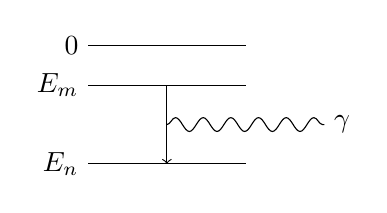
\begin{tikzpicture}
    \draw (-1, 0) node [left] {$0$} -- (1, 0);
    \draw (-1, -0.5) node [left] {$E_m$} -- (1, -0.5);
    \draw (-1, -1.5) node [left] {$E_n$} -- (1, -1.5);
    \draw [->] (0, -0.5) -- (0, -1.5);
    \draw [decorate, decoration={snake}] (0, -1) -- (2, -1) node [right] {$\gamma$};
  \end{tikzpicture}
\end{center}
This model explains a \emph{vast} amount of experimental data. This also gives an estimate of the size of a hydrogen atom:
\[
  r_1 = \left(\frac{4\pi \varepsilon_0}{me^2}\right) \hbar^2 \approx \SI{5.29e-11}{\meter},
\]
known as the \emph{Bohr radius}.

While the model fits experiments very well, it does not provide a good explanation for why the radius/angular momentum should be quantized. It simply asserts this fact and then magically produces the desired results. Thus, we would like a better understanding of why angular momentum should be quantized.

\subsection{Matter waves}
The relations
\begin{align*}
  E &= h\nu = \hbar \omega\\
  p &= \frac{h}{\lambda} = \hbar k
\end{align*}
are used to associate particle properties (energy and momentum) to waves. They can also be used the other way round --- to associate wave properties (frequency and wave number) to particles. Moreover, these apply to non-relativistic particles such as electrons (as well as relativistic photons). This $\lambda$ is known as the \emph{de Broglie wavelength}.

Of course, nothing prevents us from assigning arbitrary numbers to our particles. So an immediate question to ask is --- is there any physical significance to the ``frequency'' and ``wavenumber'' of particles? Or maybe particles in fact \emph{are} waves?

Recall that the quantization of the Bohr model requires that
\[
  L = rp = n\hbar.
\]
Using the relations above, this is equivalent to requiring that
\[
  n\lambda = 2\pi r.
\]
This is exactly the statement that the circumference of the orbit is an integer multiple of the wavelength. This is the condition we need for a standing wave to form on the circumference. This looks promising as an explanation for the quantization relation.

But in reality, do electrons actually behave like waves? If electrons really are waves, then they should exhibit the usual behaviour of waves, such as diffraction and interference.

We can repeat our favorite double-slit experiment on electrons. We have a sinusoidal wave incident on some barrier with narrow openings as shown:
\begin{center}
  \begin{tikzpicture}
    \draw (4, -2) -- (4, 2);

    \foreach \x in {-1, -2, -3} {
      \draw (\x, -2) -- (\x, 2);
    }

    \draw [<->] (-2, -1.7) -- (-3, -1.7) node [below, pos=0.5] {$\lambda$};
    \draw [->] (-3, 2.3) -- (-1.5, 2.3) node [right] {wave};

    \draw (0, 0.55) -- (4, 1.5);
    \draw (0, -0.55) -- (4, 1.5);
    \draw [domain=-2:2,samples=50, mblue] plot [smooth] ({4 + 1.5 * exp(-\x * \x) * (cos (200 * \x))^2}, \x);
    \draw [->, align=left] (4, 0) -- (6, 0) node [right] {density of\\ electrons};

    \draw [dashed] (0, 0.55) -- (0.34, -0.375);
    \node at (0.20, -0.45) [below] {$\delta$};

    \draw [mred, fill=white] (-0.05, -0.5) rectangle (0.05, 0.5);
    \draw [mred, fill=white] (-0.05, 0.6) rectangle (0.05, 2);
    \draw [mred, fill=white] (-0.05, -0.6) rectangle (0.05, -2);
  \end{tikzpicture}
\end{center}
At different points, depending on the difference $\delta$ in path length, we may have constructive interference (large amplitude) or destructive interference (no amplitude). In particular, constructive interference occurs if $\delta = n\lambda$, and destructive if $\delta = (n + \frac{1}{2})\lambda$.

Not only does this experiment allow us to verify if something is a wave. We can also figure out its wavelength $\lambda$ by experiment.

Practically, the actual experiment for electrons is slightly more complicated. Since the wavelength of an electron is rather small, to obtain the diffraction pattern, we cannot just poke holes in sheets. Instead, we need to use crystals as our diffraction grating. Nevertheless, this shows that electrons do diffract, and the wavelength \emph{is} the de Broglie wavelength.

This also has a conceptual importance. For regular waves, diffraction is something we can make sense of. However, here we are talking about electrons. We know that if we fire many many electrons, the distribution will follow the pattern described above. But what if we just fire a single electron? On \emph{average}, it should still follow the distribution. However, for this individual electron, we cannot know where it will actually land. We can only provide a probability distribution of where it will end up. In quantum mechanics, everything is inherently probabilistic.

As we have seen, quantum mechanics is vastly different from classical mechanics. This is unlike special relativity, where we are just making adjustments to Newtonian mechanics. In fact, in IA Dynamics and Relativity, we just ``derived'' special relativity by assuming the principle of relativity and that the speed of light is independent of the observer. This is not something we can do for quantum mechanics --- what we are going to do is just come up with some theory and then show (or claim) that they agree with experiment.

\section{Wavefunctions and the Schr\texorpdfstring{\"o}{o}dinger equation}
The time evolution of particles in quantum mechanics is governed by the \emph{Schr\"odinger equation}, which we will come to shortly. In general, this is a difficult equation to solve, and there aren't many interesting cases where we are able to provide a full solution.

Hence, to begin with, we will concentrate on quantum mechanics in one (spatial) dimension only, as the maths is much simpler and diagrams are easier to draw, and we can focus more on the physical content.

\subsection{Particle state and probability}
Classically, a point particle in 1 dimension has a definitive position $x$ (and momentum $p$) at each time. To completely specify a particle, it suffices to write down these two numbers. In quantum mechanics, this is much more complicated. Instead, a particle has a \emph{state} at each time, specified by a complex-valued \emph{wavefunction} $\psi(x)$.

The physical content of the wavefunction is as follows: if $\psi$ is appropriately normalized, then when we measure the position of a particle, we get a result $x$ with probability density function $|\psi(x)|^2$, i.e.\ the probability that the position is found in $[x, x + \delta x]$ (for small $\delta x$) is given by $|\psi(x)|^2 \delta x$. Alternatively, the probability of finding it in an interval $[a, b]$ is given by
\[
  \P(\text{particle position in }[a, b]) = \int_a^b |\psi(x)|^2 \;\d x.
\]
What do we mean by ``appropriately normalized''? From our equation above, we see that we require
\[
  \int_{-\infty}^\infty |\psi(x)|^2\;\d x = 1,
\]
since this is the total probability of finding the particle anywhere at all. This the normalization condition required.

\begin{eg}[Gaussian wavefunction]
  We define
  \[
    \psi(x) = C e^{-\frac{(x - c)^2}{2\alpha}},
  \]
  where $c$ is real and $C$ could be complex.
  \begin{center}
    \begin{tikzpicture}[yscale=1.5]
      \draw (-3, 0) -- (3, 0);
      \draw (0, 1.3) -- (0, 0) node [below] {$c$};
      \draw [domain=-3:3,samples=50, mblue] plot (\x, {exp(-\x * \x)});
    \end{tikzpicture}
  \end{center}
  We have
  \[
    \int_{-\infty}^\infty |\psi(x)|^2 \;\d x = |C|^2 \int_{-\infty}^{\infty}e^{-\frac{(x - c)^2}{\alpha}} \;\d x = |C|^2 (\alpha \pi)^{\frac{1}{2}} = 1.
  \]
  So for normalization, we need to pick $C = (1/\alpha \pi)^{1/4}$ (up to a multiple of $e^{i\theta}$).

  If $\alpha$ is small, then we have a sharp peak around $x = c$. If $\alpha$ is large, it is more spread out.
\end{eg}
While it is nice to have a normalized wavefunction, it is often inconvenient to deal exclusively with normalized wavefunctions, or else we will have a lot of ugly-looking constants floating all around. As a matter of fact, we can always restore normalization at the end of the calculation. So we often don't bother.

If we do not care about normalization, then for any (non-zero) $\lambda$, $\psi(x)$ and $\lambda \psi(x)$ represent the same quantum state (since they give the same probabilities). In practice, we usually refer to either of these as ``the state''. If we like fancy words, we can thus think of the states as equivalence classes of wavefunctions under the equivalence relation $\psi \sim \phi$ if $\phi = \lambda \psi$ for some non-zero $\lambda$.

What we do require, then, is not that the wavefunction is normalized, but \emph{normalizable}, i.e.
\[
  \int_{-\infty}^\infty |\psi(x)|^2 \;\d x < \infty.
\]
We will very soon encounter wavefunctions that are \emph{not} normalizable. Mathematically, these are useful things to have, but we have to be more careful when interpreting these things physically.

A characteristic property of quantum mechanics is that if $\psi_1(x)$ and $\psi_2(x)$ are wavefunctions for a particle, then $\psi_1(x) + \psi_2 (x)$ is also a possible particle state (ignoring normalization), provided the result is non-zero. This is the principle of superposition, and arises from the fact that the equations of quantum mechanics are linear.

\begin{eg}[Superposition of Gaussian wavefunctions]
  Take
  \[
    \psi(x) = B\left(\exp\left(\frac{-(x - c)^2}{2\alpha}\right) + \exp\left(-\frac{x^2}{2\beta}\right)\right).
  \]
  Then the resultant distribution would be something like
  \begin{center}
    \begin{tikzpicture}[xscale=0.75, yscale=1.5]
      \draw (-3, 0) -- (9, 0);
      \draw [domain=-3:9,samples=80, mblue] plot (\x, {exp(-\x * \x) + exp(-(\x - 6)^2/4)});
    \end{tikzpicture}
  \end{center}
  We choose $B$ so that $\psi$ in a normalized wavefunction for a single particle. Note that this is \emph{not} two particles at two different positions. It is \emph{one} particle that is ``spread out'' at two different positions.
\end{eg}
It is possible that in some cases, the particles in the configuration space may be restricted. For example, we might require $ -\frac{\ell}{2} \leq x \leq \frac{\ell}{2}$ with some boundary conditions at the edges. Then the normalization condition would not be integrating over $(-\infty, \infty)$, but $[-\frac{\ell}{2}, \frac{\ell}{2}]$.

\subsection{Operators}
We know that the square of the wavefunction gives the probability distribution of the \emph{position} of the particle. How about other information such as the momentum and energy? It turns out that all the information about the particle is contained in the wavefunction (which is why we call it the ``state'' of the particle).

We call each property of the particle which we can measure an \emph{observable}. Each observable is represented by an \emph{operator} acting on $\psi(x)$. For example, the position is represented by the operator $\hat{x} = x$. This means that $(\hat{x} \psi)(x) = x\psi(x)$. We can list a few other operators:
\begin{center}
  \begin{tabular}{rll}
    position & $\hat{x} = x$ & $\hat{x} \psi = x\psi(x)$\\
    momentum & $\hat{p} = -i\hbar \frac{\partial}{\partial x}$ & $\hat{p}\psi = -i\hbar \psi'(x)$\\
    energy & $H = \frac{\hat{p}^2}{2m} + V(\hat{x})$ & $H\psi = -\frac{\hbar^2}{2m} \frac{\partial^2}{\partial x^2}\psi + V(x)\psi(x)$
  \end{tabular}
\end{center}
The final $H$ is called the Hamiltonian, where $m$ is the mass and $V$ is the potential. We see that the Hamiltonian is just the kinetic energy $\frac{p^2}{2m}$ and the potential energy $V$. There will be more insight into why the operators are defined like this in IIC Classical Dynamics and IID Principles of Quantum Mechanics.

Note that we put hats on $\hat{x}$ and $\hat{p}$ to make it explicit that these are operators, as opposed to the classical quantities position and momentum. Otherwise, the definition $\hat{x} = x$ would look silly.

How do these operators relate to the actual physical properties? In general, when we measure an observable, the result is not certain. They are randomly distributed according to some probability distribution, which we will go into full details later.

However, a \emph{definite} result is obtained if and only if $\psi$ is an eigenstate, or eigenfunction, of the operator. In this case, results of the measurements are the eigenvalue associated. For example, we have
\[
  \hat{p} \psi = p\psi
\]
if and only if $\psi$ is a state with definite momentum $p$. Similarly,
\[
  H\psi = E\psi
\]
if and only if $\psi$ has definite energy $E$.

Here we are starting to see why quantization occurs in quantum mechanics. Since the only possible values of $E$ and $p$ are the eigenvalues, if the operators have a discrete set of eigenvalues, then we can only have discrete values of $p$ and $E$.

\begin{eg}
  Let
  \[
    \psi(x) = Ce^{ikx}.
  \]
  This has a wavelength of $\lambda = 2\pi/k$. This is a momentum eigenstate, since we have
  \[
    \hat{p}\psi = -\hbar \psi' = (\hbar k)\psi.
  \]
  So we know that the momentum eigenvalue is $p = \hbar k$. This looks encouraging!

  Note that if there is no potential, i.e.\ $V = 0$, then
  \[
    H\psi = \frac{\hat{p}^2}{2m}\psi = -\frac{\hbar^2}{2m}\psi'' = \frac{\hbar^2 k^2}{2m}\psi.
  \]
  So the energy eigenvalue is
  \[
    E = \frac{\hbar^2 k^2}{2m}.
  \]
\end{eg}
Note, however, that our wavefunction has $|\psi(x)|^2 = |C|^2$, which is a constant. So this wavefunction is not normalizable on the whole line. However, if we restrict ourselves to some finite domain $-\frac{\ell}{2} \leq x \leq \frac{\ell}{2}$, then we can normalize by picking $C= \frac{1}{\sqrt{\ell}}$.

\begin{eg}
  Consider the Gaussian distribution
  \[
    \psi(x) = C\exp\left(-\frac{x^2}{2\alpha}\right).
  \]
  We get
  \[
    \hat{p}\psi(x) = -i\hbar \psi'(x) \not= p\psi(x)
  \]
  for any number $p$. So this is not an eigenfunction of the momentum.

  However, if we consider the harmonic oscillator with potential
  \[
    V(x) = \frac{1}{2}Kx^2,
  \]
  then this $\psi(x)$ is an eigenfunction of the Hamiltonian operator, provided we picked the right $\alpha$. We have
  \[
    H\psi = -\frac{\hbar^2}{2m}\psi'' + \frac{1}{2}Kx^2 \psi = E\psi
  \]
  when $\alpha^2 = \frac{\hbar^2}{Km}$. Then the energy is $E = \frac{\hbar}{2}\sqrt{\frac{K}{m}}$. This is to be verified on the example sheet.
\end{eg}
Despite being a simple system, the harmonic oscillator is \emph{incredibly} useful in theoretical physics. We will hence solve this completely later.

\begin{defi}[Time-independent Schr\"odinger equation]
  The \emph{time-independent Schr\"odinger equation} is the energy eigenvalue equation
  \[
    H\psi = E\psi,
  \]
  or
  \[
    -\frac{\hbar^2}{2m}\psi'' + V(x) \psi = E\psi.
  \]
\end{defi}
This is in general what determines what the system behaves. In particular, the eigenvalues $E$ are precisely the allowed energy values.

\subsection{Time evolution of wavefunctions}
So far, everything is instantaneous. The wavefunction specifies the state \emph{at a particular time}, and the eigenvalues are the properties of the system \emph{at that particular time}. However, this is quantum \emph{mechanics}, or quantum \emph{dynamics}. We should be looking at how things \emph{change}. We want to know how the wavefunction changes with time. This is what we will get to now.

\subsubsection*{Time-dependent Schr\"odinger equation}
We will write $\Psi$ instead of $\psi$ to indicate that we are looking at the time-dependent wavefunction. The evolution of this $\Psi(x, t)$ is described by the time-dependent Schr\"odinger equation.
\begin{defi}[Time-dependent Schr\"odinger equation]
  For a time-dependent wavefunction $\Psi(x, t)$, the \emph{time-dependent Schr\"odinger equation} is
  \[
    i\hbar \frac{\partial \Psi}{\partial t} = H\Psi.\tag{$*$}
  \]
\end{defi}
For a particle in a potential $V(x)$, this can reads
\[
  i\hbar \frac{\partial \Psi}{\partial t} = -\frac{\hbar^2}{2m}\frac{\partial^2 \Psi}{\partial x^2} + V(x) \Psi.
\]
While this looks rather scary, it isn't really that bad. First of all, it is linear. So the sums and multiples of solutions are also solutions. It is also first-order in time. So if we know the wavefunction $\Psi(x, t_0)$ at a particular time $t_0$, then this determines the whole function $\Psi(x, t)$.

This is similar to classical dynamics, where knowing the potential $V$ (and hence the Hamiltonian $H$) completely specifies how the system evolves with time. However, this is in some ways different from classical dynamics. Newton's second law is second-order in time, while this is first-order in time. This is significant since when our equation is first-order in time, then the current state of the wavefunction completely specifies the evolution of the wavefunction in time.

Yet, this difference is just an illusion. The wavefunction is the \emph{state} of the particle, and not just the ``position''. Instead, we can think of it as capturing the position \emph{and} momentum. Indeed, if we write the equations of classical dynamics in terms of position and momentum, it will be first order in time.

\subsubsection*{Stationary states}
It is not the coincidence that the time-independent Schr\"odinger equation and the time-dependent Schr\"odinger equation are named so similarly (and it is also not an attempt to confuse students).

We perform separation of variables, and consider a special class of solutions $\Psi(x, t) = T(t) \psi(x)$, where $\Psi(x, 0) = \psi(x)$ (i.e.\ $T(0) = 1$). If $\psi$ satisfies the time-independent Schr\"odinger equation
\[
  H\psi = E\psi,
\]
then since $H$ does not involve time derivatives, we know $\Psi$ is an energy eigenstate at each fixed $t$, i.e.
\[
  H\Psi = E\Psi.
\]
So if we want this $\Psi$ to satisfy the Schr\"odinger equation, we must have
\[
  i\hbar \dot{T} = ET.
\]
The solution is obvious:
\[
  T(t) = \exp\left(-\frac{iEt}{\hbar}\right).
\]
We can write our full solution as
\[
  \Psi(x, t) = \psi(x) \exp\left(-\frac{iEt}{\hbar}\right).
\]
Note that the frequency is $\omega = \frac{E}{\hbar}$. So we recover the Energy-frequency relation we've previously had.

\begin{defi}[Stationary state]
  A \emph{stationary state} is a state of the form
  \[
    \Psi(x, t) = \psi(x) \exp\left(-\frac{iEt}{\hbar}\right).
  \]
  where $\psi(x)$ is an eigenfunction of the Hamiltonian with eigenvalue $E$. This term is also sometimes applied to $\psi$ instead.
\end{defi}
While the stationary states seem to be a rather peculiar class of solutions that would rarely correspond to an actual physical state in reality, they are in fact very important in quantum mechanics. The reason is that the stationary states form a \emph{basis} of the state space. In other words, every possible state can be written as a (possibly infinite) linear combination of stationary states. Hence, by understanding the stationary states, we can understand a lot about a quantum system.

\subsubsection*{Conservation of probability}
Note that for a stationary state, we have
\[
  |\Psi(x, t)|^2 = |\psi(x)|^2,
\]
which is independent of time. In general, this is true in most cases.

Consider a general $\Psi(x, t)$ obeying the time-dependent Schr\"odinger equation.

\begin{prop}
  The probability density
  \[
    P(x, t) = |\Psi(x, t)|^2
  \]
  obeys a conservation equation
  \[
    \frac{\partial P}{\partial t} = - \frac{\partial j}{\partial x},
  \]
  where
  \[
    j(x, t) = -\frac{i\hbar}{2m} \left(\Psi^*\frac{\d \Psi}{\d x} - \frac{\d \Psi^*}{\d x} \Psi\right)
  \]
  is the \emph{probability current}.
\end{prop}
Since $\Psi^* \Psi'$ is the complex conjugate of $\Psi'^* \Psi$, we know that $\Psi^*\Psi' - \Psi'^* \Psi$ is imaginary. So multiplying by $i$ ensures that $j(x, t)$ is real, which is a good thing since $P$ is also real.

\begin{proof}
  This is straightforward from the Schr\"odinger equation and its complex conjugate. We have
  \begin{align*}
    \frac{\partial P}{\partial t} &= \Psi^* \frac{\partial \Psi}{\partial t} + \frac{\partial \Psi*}{\partial t} \Psi\\
    &= \Psi^* \frac{i\hbar }{2m}\Psi'' - \frac{i\hbar}{2m}\Psi''^* \Psi\\
    \intertext{where the two $V$ terms cancel each other out, assuming $V$ is real}
    &= -\frac{\partial j}{\partial x}.\qedhere
  \end{align*}
\end{proof}
The important thing here is not the specific form of $j$, but that $\frac{\partial P}{\partial t}$ can be written as the space derivative of some quantity. This implies that the probability that we find the particle in $[a, b]$ at fixed time $t$ changes as
\[
  \frac{\d}{\d t}\int_a^b |\Psi(x, t)|^2 \;\d x = \int_a^b -\frac{\partial j}{\partial x}(x, t)\;\d x = j(a, t) - j(b, t).
\]
We can think of the final term as the probability current getting in and out of the interval at the boundary.

In particular, consider a normalizable state with $\Psi, \Psi', j \to 0$ as $x \to \pm\infty$ for fixed $t$. Taking $a \to -\infty$ and $b\to +\infty$, we have
\[
  \frac{\d}{\d t}\int_{-\infty}^\infty |\Psi(x, t)|^2 \;\d x = 0.
\]
What does this tell us? This tells us that if $\Psi(x, 0)$ is normalized, $\Psi(x, t)$ is normalized for all $t$. Hence we know that for each fixed $t$, $|\Psi(x, t)|^2$ is a probability distribution. So what this really says is that the probability interpretation is consistent with the time evolution.

\section{Some examples in one dimension}
\subsection{Introduction}
In general, we are going to consider the energy eigenvalue problem for a particle in 1 dimension in a potential $V(x)$, i.e.
\[
  H\psi = -\frac{\hbar^2}{2m}\psi'' + V(x) \psi = E\psi.
\]
In other words, we want to find the allowed energy eigenvalues.

This is a hard problem in general. However, we can consider the really easy case where $V(X) = U$, where $U$ is a constant. Then we can easily write down solutions.

If $U > E$, then the Schr\"odinger equation is equivalent to
\[
  \psi'' - \kappa^2 \psi = 0,
\]
where $\kappa$ is such that $U - E = \frac{\hbar^2 \kappa^2}{2m}$. We take wlog $\kappa > 0$. The solution is then
\[
  \psi = Ae^{\kappa x} + Be^{-\kappa x}.
\]
On the other hand, if $U < E$, then the Schr\"odinger equation says
\[
  \psi + k^2 \psi = 0,
\]
where $k$ is picked such that $E - U = \frac{\hbar^2 k^2}{2m}$. The solutions are
\[
  \psi = Ae^{ikx} + Be^{ikx}.
\]
Note that these new constants are merely there to simplify our equations. They generally need not have physical meanings.

Now why are we interested in cases where the potential is constant? Wouldn't that be just equivalent to a free particle? This is indeed true. However, knowing these solutions allow us to to study piecewise flat potentials such as steps, wells and barriers.
\begin{center}
  \begin{tikzpicture}
    \begin{scope}
      \draw [->] (-1.5, 0) -- (1.5, 0) node [right] {$x$};
      \draw [->] (0, -0.5) -- (0, 1.5) node [above] {$V$};
      \draw [mred, semithick] (-1.5, 0) -- (0, 0) -- (0, 1) -- (1, 1);
    \end{scope}

    \begin{scope}[shift={(4, 0)}]
      \draw [->] (-1.5, 0) -- (1.5, 0) node [right] {$x$};
      \draw [->] (0, -0.5) -- (0, 1.5) node [above] {$V$};
      \draw [mred, semithick] (-1.5, 1) -- (-0.5, 1) -- (-0.5, 0) -- (0.5, 0) -- (0.5, 1) -- (1.5, 1);
    \end{scope}

    \begin{scope}[shift={(8, 0)}]
      \draw [->] (-1.5, 0) -- (1.5, 0) node [right] {$x$};
      \draw [->] (0, -0.5) -- (0, 1.5) node [above] {$V$};
      \draw [mred, semithick] (-1.5, 0) -- (-0.5, 0) -- (-0.5, 1) -- (0.5, 1) -- (0.5, 0) -- (1.5, 0);
    \end{scope}
  \end{tikzpicture}
\end{center}
Here a finite discontinuity in $V$ is allowed. In this case, we can have $\psi, \psi'$ continuous and $\psi''$ discontinuous. Then the discontinuity of $\psi''$ cancels that of $V$, and the Schr\"odinger equation holds everywhere.

In this chapter, we will seek normalizable solutions with
\[
  \int_{-\infty}^\infty |\psi(x)|^2 \;\d x.
\]
This requires that $\psi(x) \to 0$ as $x \to \pm\infty$. We see that for the segments and the end, we want to have decaying exponentials $e^{-\kappa x}$ instead of oscillating exponentials $e^{-ikx}$.

\subsection{Infinite well --- particle in a box}
The simplest case to consider is the infinite well. Here the potential is infinite outside the region $[-a, a]$, and we have much less to think about. For $|x| > a$, we must have $\psi(x) = 0$, or else $V(x) \psi(x)$ would be infinite.
\begin{center}
  \begin{tikzpicture}
    \draw [->] (-2.5, 0) -- (2.5, 0) node [right] {$x$};
    \draw [->] (0, -0.5) -- (0, 2) node [above] {$V$};
    \draw [mred, semithick, ->] (-1.5, 0) node [below] {$-a$} -- (-1.5, 2);
    \draw [mred, semithick, ->] (1.5, 0) node [below] {$a$} -- (1.5, 2);
    \draw [mred, semithick] (-1.5, 0) -- (1.5, 0);
  \end{tikzpicture}
\end{center}
\[
  V(x) =
  \begin{cases}
    0 & |x| \leq a\\
    \infty & |x| > a.
  \end{cases}
\]
We require $\psi = 0$ for $|x| > a$ and $\psi$ continuous at $x = \pm a$. Within $|x| < a$, the Schr\"odinger equation is
\[
  -\frac{\hbar^2}{2m}\psi'' = E\psi.
\]
We simplify this to become
\[
  \psi'' + k^2 \psi = 0,
\]
where
\[
  E = \frac{\hbar^2 k^2}{2m}.
\]
Here, instead of working with the complex exponentials, we use $\sin$ and $\cos$ since we know well when these vanish. The general solution is thus
\[
  \psi = A\cos kx + B\sin kx.
\]
Our boundary conditions require that $\psi$ vanishes at $x = \pm a$. So we need
\[
  A \cos ka \pm B\sin ka = 0.
\]
In other words, we require
\[
  A\cos ka = B\sin ka = 0.
\]
Since $\sin ka$ and $\cos ka$ cannot be simultaneously $0$, either $A = 0$ or $B = 0$. So the two possibilities are
\begin{enumerate}
  \item $B = 0$ and $ka = n\pi/2$ with $n = 1, 3, \cdots$
  \item $A = 0$ and $ka = n\pi/2$ with $n = 2, 4, \cdots$
\end{enumerate}
Hence the allowed energy levels are
\[
  E_n = \frac{\hbar^2 \pi^2}{8ma^2} n^2,
\]
where $n = 1, 2, \cdots$, and the wavefunctions are
\[
  \psi_n(x) = \left(\frac{1}{a}\right)^{\frac{1}{2}}
  \begin{cases}
    \cos \frac{n\pi x}{2a} & n\text{ odd}\\
    \sin \frac{n\pi x}{2a} & n\text{ even}
  \end{cases}.
\]
These are normalized with $\int_{-a}^a |\psi_n(x)|^2 \;\d x$.
\begin{center}
  \begin{tikzpicture}
    \begin{scope}
      \node [right] at (-2.5, 1.5) {$\psi_1$:};
      \draw [->] (-2.5, 0) -- (2.5, 0) node [right] {$x$};
      \draw [->] (0, -1.5) -- (0, 1.5) node [above] {$V$};
      \node [anchor = north east] at (-1.5, 0) {$-a$};
      \node [anchor = north west] at (1.5, 0) {$-a$};
      \draw [mred] (-1.5, -1.5) -- (-1.5, 1.5);
      \draw [mred] (1.5, -1.5) -- (1.5, 1.5);

      \draw [mblue, semithick, domain=-1.5:1.5, samples=50] plot (\x, {cos (60 * \x)});
    \end{scope}

    \begin{scope}[shift={(6, 0)}]
      \node [right] at (-2.5, 1.5) {$\psi_2$:};
      \draw [->] (-2.5, 0) -- (2.5, 0) node [right] {$x$};
      \draw [->] (0, -1.5) -- (0, 1.5) node [above] {$V$};
      \node [anchor = north east] at (-1.5, 0) {$-a$};
      \node [anchor = north west] at (1.5, 0) {$-a$};
      \draw [mred] (-1.5, -1.5) -- (-1.5, 1.5);
      \draw [mred] (1.5, -1.5) -- (1.5, 1.5);

      \draw [mblue, semithick, domain=-1.5:1.5, samples=50] plot (\x, {sin (120 * \x)});
    \end{scope}

    \begin{scope}[shift={(0, -4)}]
      \node [right] at (-2.5, 1.5) {$\psi_3$:};
      \draw [->] (-2.5, 0) -- (2.5, 0) node [right] {$x$};
      \draw [->] (0, -1.5) -- (0, 1.5) node [above] {$V$};
      \node [anchor = north east] at (-1.5, 0) {$-a$};
      \node [anchor = north west] at (1.5, 0) {$-a$};
      \draw [mred] (-1.5, -1.5) -- (-1.5, 1.5);
      \draw [mred] (1.5, -1.5) -- (1.5, 1.5);

      \draw [mblue, semithick, domain=-1.5:1.5, samples=50] plot (\x, {cos (180 * \x)});
    \end{scope}

    \begin{scope}[shift={(6, -4)}]
      \node [right] at (-2.5, 1.5) {$\psi_4$:};
      \draw [->] (-2.5, 0) -- (2.5, 0) node [right] {$x$};
      \draw [->] (0, -1.5) -- (0, 1.5) node [above] {$V$};
      \node [anchor = north east] at (-1.5, 0) {$-a$};
      \node [anchor = north west] at (1.5, 0) {$-a$};
      \draw [mred] (-1.5, -1.5) -- (-1.5, 1.5);
      \draw [mred] (1.5, -1.5) -- (1.5, 1.5);

      \draw [mblue, semithick, domain=-1.5:1.5, samples=50] plot (\x, {sin (240 * \x)});
    \end{scope}
  \end{tikzpicture}
\end{center}
This was a rather simple and nice example. We have an infinite well, and the particle is well-contained inside the box. The solutions just look like standing waves on a string with two fixed end points --- something we (hopefully) are familiar with.

Note that $\psi_n(-x) = (-1)^{n + 1}\psi_n(x)$. We will see that this is a general feature of energy eigenfunctions of a symmetric potential. This is known as \emph{parity}.
\subsection{Parity}
Consider the Schr\"odinger equation for a particle of mass $m$
\[
  H\psi = -\frac{\hbar^2}{2m}\psi'' + V(x) \psi = E\psi.
\]
with potential
\[
  V(x) = V(-x).
\]
By changing variables $x \to -x$, we see that $\psi(x)$ is an eigenfunction of $H$ with energy $E$ if and only if $\psi(-x)$ is an eigenfunction of $H$ with energy $E$. There are two possibilities:
\begin{enumerate}
  \item If $\psi(x)$ and $\psi(-x)$ represent the same quantum state, this can only happen if $\psi(-x) = \eta \psi(x)$ for some constant $\eta$. Since this is true for all $x$, we can do this twice and get
    \[
      \psi(x) = \eta \psi(-x) = \eta^2 \psi(x).
    \]
    So we get that $\eta = \pm 1$ and $\psi(-x) = \pm \psi(x)$. We call $\eta$ the \emph{parity}, and say $\psi$ has even/odd parity if $\eta$ is $+1/-1$ respectively.

    For example, in our particle in a box, our states $\psi_n$ have parity $(-1)^{n + 1}$.
  \item If $\psi(x)$ and $\psi(-x)$ represent different quantum states, then we can still take linear combinations
    \[
      \psi_\pm (x) = \alpha(\psi(x) \pm \psi(-x)),
    \]
    and these are also eigenstates with energy eigenvalue $E$, where $\alpha$ is for normalization. Then by construction, $\psi_\pm (-x) = \pm \psi_\pm(x)$ and have parity $\eta = \pm 1$.
\end{enumerate}
Hence, if we are given a potential with reflective symmetry $V(-x) = V(x)$, then we can restrict our attention and just look for solutions with definite parity.
\subsection{Potential well}
We will consider a potential that looks like this:
\begin{center}
  \begin{tikzpicture}[scale=1.5]
    \draw [->] (-1.5, 0) -- (1.5, 0) node [right] {$x$};
    \draw [->] (0, -1.5) -- (0, 0.5) node [above] {$V$};
    \draw [mred, semithick] (-1.5, 0) -- (-0.5, 0) -- (-0.5, -1) node [below] {$-a$} -- (0.5, -1) node [below] {$a$} -- (0.5, 0) -- (1.5, 0);

    \draw [dashed] (0.5, -1) -- (1.5, -1) node [right] {$-U$};
  \end{tikzpicture}
\end{center}
The potential is given by
\[
  V(x) =
  \begin{cases}
    -U & |x| < a\\
    0 & |x| \geq a
  \end{cases}
\]
for some constant $U > 0$. Classically, this is not very interesting. If the energy $E < 0$, then the particle is contained in the well. Otherwise it is free to move around. However, in quantum mechanics, this is much more interesting.

We want to seek energy levels for a particle of mass $m$, defined by the Schr\"odinger equation
\[
  H\psi = -\frac{\hbar^2}{2m}\psi'' + V(x) \psi = E\psi.
\]
For energies in the range
\[
  -U < E < 0,
\]
we set
\[
  U + E = \frac{\hbar^2 k^2}{2m} > 0,\quad E = -\frac{\hbar^2 \kappa^2}{2m},
\]
where $k, \kappa > 0$ are new real constants. Note that these coefficients are not independent, since $U$ is given and fixed. So they must satisfy
\[
  k^2 + \kappa^2 = \frac{2mU}{\hbar^2}.
\]
Using these constants, the Schr\"odinger equation becomes
\[
  \begin{cases}
    \psi'' + k^2 \psi = 0 & |x| < a\\
    \psi'' - \kappa^2 \psi = 0 & |x| > a.
  \end{cases}
\]
As we previously said, we want the Schr\"odinger equation to hold even at the discontinuities. So we need $\psi$ and $\psi'$ to be continuous at $x = \pm a$.

We first consider the even parity solutions $\psi(-x) = \psi(x)$. We can write our solution as
\[
  \psi =
  \begin{cases}
    A \cos kx & |x| < a\\
    B e^{-\kappa |x|} & |x| > a\\
  \end{cases}
\]
We match $\psi$ and $\psi'$ at $x = a$. So we need
\begin{align*}
  A\cos ka &= Be^{-\kappa a}\\
  -Ak\sin ka &= -\kappa Be^{-\kappa a}.
\end{align*}
By parity, there is no additional information from $x = -a$.

We can divide the equations to obtain
\[
  k \tan ka = \kappa.
\]
this is still not something we can solve easily. To find when solutions exist, it is convenient to introduce
\[
  \xi = ak, \quad \eta = a\kappa,
\]
where these two constants are dimensionless and positive. Note that this $\eta$ has nothing to do with parity. It's just that we have run out of letters to use. Hence the solution we need are solutions to
\[
  \eta = \xi \tan \xi.
\]
Also, our initial conditions on $k$ and $\kappa$ require
\[
  \xi^2 + \eta^2 = \frac{2ma^2 U}{\hbar^2}.
\]
We can look for solutions by plotting these two equations. We first plot the curve $\eta = \xi \tan \xi$:
\begin{center}
  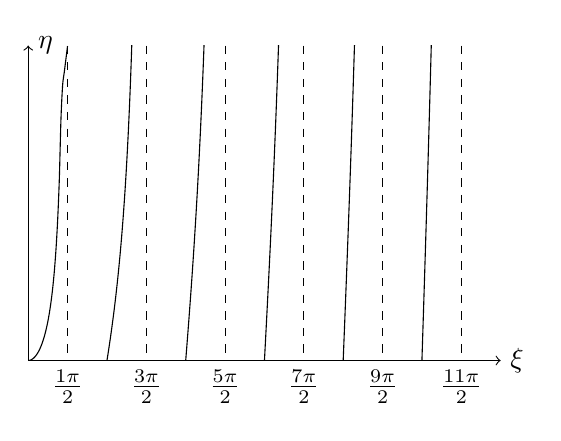
\begin{tikzpicture}
    \draw [->] (0, 0) -- (6, 0) node [right] {$\xi$};
    \draw [->] (0, 0) -- (0, 4) node [right] {$\eta$};
    \begin{scope}[yscale=2]
      \clip (0, 0) rectangle (6, 2);
      \foreach \a in {0,1,...,5} {
        \pgfmathsetmacro\b{\a + 0.499};
        \draw [domain=\a:\b] plot [smooth] (\x, {\x * min(4, tan(180*\x))});
      }
    \end{scope}
    \foreach \a in {0,1,...,5} {
        \pgfmathsetmacro\n{\a * 2 + 1};
      \draw [dashed] (\a + 0.5, 4) -- (\a + 0.5, 0) node [below] {$\frac{\pgfmathprintnumber{\n} \pi}{2}$};
    }
  \end{tikzpicture}
\end{center}
The other equation is the equation of a circle. Depending on the size of the constant $2ma^2 U/\hbar^2$, there will be a different number of points of intersections.
\begin{center}
  \begin{tikzpicture}
    \draw [->] (0, 0) -- (6, 0) node [right] {$\xi$};
    \draw [->] (0, 0) -- (0, 4) node [right] {$\eta$};
    \begin{scope}[yscale=2]
      \clip (0, 0) rectangle (6, 2);
      \foreach \a in {0,1,...,5} {
        \pgfmathsetmacro\b{\a + 0.499};
        \draw [domain=\a:\b] plot [smooth] (\x, {\x * min(4, tan(180*\x))});
      }
    \end{scope}
    \draw [mred, dashed] (2.3, 0) arc (0:90:2.3);
    \draw [mred, dashed] (1.5, 0) arc (0:90:1.5);
  \end{tikzpicture}
\end{center}
So there will be a different number of solutions depending on the value of $2ma^2 U/\hbar^2$. In particular, if
\[
  (n - 1)\pi < \left(\frac{2mUa^2}{\hbar^2}\right)^{1/2} < n\pi,
\]
then we have exactly $n$ even parity solutions (for $n \geq 1$).

We can do exactly the same thing for odd parity eigenstates\ldots on example sheet 1.

For $E > 0$ or $E < -U$, we will end up finding non-normalizable solutions. What is more interesting, though is to look at the solutions we have now. We can compare what we've got with what we would expect classically.

Classically, any value of $E$ in the range $-U < E < 0$ is allowed, and the motion is deeply uninteresting. The particle just goes back and forth inside the well, and is \emph{strictly confined} in $-a \leq x \leq a$.

Quantum mechanically, there is just a discrete, \emph{finite} set of allowed energies. What is more surprising is that while $\psi$ decays exponentially outside the well, it is non-zero! This means there is in theory a non-zero probability of finding the particle outside the well! We call these particles \emph{bound} in the potential, but in fact there is a non-zero probability of finding the particle outside the well.

\subsection{The harmonic oscillator}
So far in our examples, the quantization (mathematically) comes from us requiring continuity at the boundaries. In the harmonic oscillator, it arises in a different way.
\begin{center}
  \begin{tikzpicture}[scale=1.5]
    \draw [->] (-1.5, 0) -- (1.5, 0) node [right] {$x$};
    \draw [->] (0, -0.5) -- (0, 1.5) node [above] {$V$};
    \draw [mred, semithick] (-1, 1.5) parabola bend (0, 0) (1, 1.5);
  \end{tikzpicture}
\end{center}
This is a harmonic oscillator of mass $m$ with
\[
  V(x) = \frac{1}{2}m\omega^2 x^2.
\]
Classically, this has a motion of $x = A \cos \omega (t - t_0)$, which is something we (hopefully) know well too.

This is a \emph{really} important example. First of all, we can solve it, which is a good thing. More importantly, any smooth potential can be approximated by a harmonic oscillator near an equilibrium $x_0$, since
\[
  V(x) = V(x_0) + \frac{1}{2}V''(x_0)(x - x_0)^2 + \cdots.
\]
Systems with many degrees like crystals can also be treated as collections of independent oscillators by considering the normal modes. If we apply this to the electromagnetic field, we get photons! So it is very important to understand the quantum mechanical oscillator.

We are going to seek all normalizable solutions to the time-independent Schr\"odinger equation
\[
  H\psi = -\frac{\hbar^2}{2m}\psi'' + \frac{1}{2}m\omega^2 x^2 \psi = E\psi.
\]
So simplify constants, we define
\[
  y = \left(\frac{m\omega}{\hbar}\right)^{\frac{1}{2}}x,\quad \mathcal{E} = \frac{2E}{\hbar \omega},
\]
both of which is dimensionless. Then we are left with
\[
  -\frac{\d^2 \psi}{\d y^2} + y^2\psi = \mathcal{E} \psi.
\]
We can consider the behaviour for $y^2 \gg \mathcal{E}$. For large $y$, the $y^2 \psi$ term will be large, and so we want the $\psi''$ term to offset it. We might want to try the Gaussian $e^{-y^2/2}$, and when we differentiate it twice, we would have brought down a factor of $y^2$. So we can wlog set
\[
  \psi = f(y) e^{-\frac{1}{2}y^2}.
\]
Then the Schr\"odinger equation gives
\[
  \frac{\d^2 f}{\d y^2} - 2y\frac{\d f}{\d y} + (\mathcal{E} - 1) = 0.
\]
This is known as \emph{Hermite's equation}. We try a series solution
\[
  f(y) = \sum_{r \geq 0} a_r y^r,
\]
and substitute in to get
\[
  \sum_{r \geq 0} \big( (r + 2)(r + 1)a_{n + 2} + (\mathcal{E} - 1 - 2r)a_r\big) y^r = 0.
\]
This holds if and only if
\[
  a_{r + 2} = \frac{2 r + 1 - \mathcal{E}}{(r + 2)(r + 1)} a_r,\quad r \geq 0.
\]
We can choose $a_0$ and $a_1$ independently, and can get two linearly independent solutions. Each solution involves either all even or all odd powers.

However, we have a problem. We want normalizable solutions. So we want to make sure our function does not explode at large $y$. Note that it is okay if $f(y)$ is \emph{quite} large, since our $\psi$ is suppressed by the $e^{-\frac{1}{2}y^2}$ terms, but we cannot grow \emph{too} big.

We look at these two solutions individually. To examine the behaviour of $f(y)$ when $y$ is large, observe that unless the coefficients vanish, we get
\[
  a_{p}/a_{p - 2} \sim \frac{1}{p}.
\]
This matches the coefficients of $y^\alpha e^{y^2}$ for some power $\alpha$ (e.g.\ $\sum_{p \geq 0} \frac{y^{2p}}{p!}$). This is bad, since our $\psi$ will then grow as $e^{\frac{1}{2}y^2}$, and cannot be normalized.

Hence, we get normalizable $\psi$ if and only if the series for $f$ terminates to give a polynomial. This occurs iff $\mathcal{E} = 2n + 1$ for some $n$. Note that for each $n$, only one of the two independent solutions is normalizable. So for each $\mathcal{E}$, we get exactly one solution.

So for $n$ even, we have
\[
  a_{r + 2} = \frac{2r - 2n}{(r + 2)(r + 1)} a_r
\]
for $r$ even, and $a_r = 0$ for $r$ odd, and the other way round when $n$ is odd.

The solutions are thus $f(y) = h_n(y)$, where $h_n$ is a polynomial of degree $n$ with $h_n(-y) = (-1)^n h_n(y)$.

For example, we have
\begin{align*}
  h_0(y) &= a_0\\
  h_1(y) &= a_1 y\\
  h_2(y) &= a_0(1 - 2y^2)\\
  h_3(y) &= a_1\left(y - \frac{2}{3}y^3\right).
\end{align*}
These are known as the \emph{Hermite polynomials}. We have now solved our harmonic oscillator. With the constant restored, the possible energy eigenvalues are
\[
  E_n = \hbar \omega \left(n + \frac{1}{2}\right),
\]
for $n = 0, 1, 2, \cdots$.

The wavefunctions are
\[
  \psi_n(x) = h_n \left(\left(\frac{m\omega}{\hbar}\right)^{\frac{1}{2}} x\right) \exp\left(-\frac{1}{2}\frac{m\omega}{\hbar} x^2\right),
\]
where normalization fixes $a_0$ and $a_1$.

As we said in the beginning, harmonic oscillators are everywhere. It turns out quantised electromagnetic fields correspond to sums of quantised harmonic oscillators, with
\[
  E_n - E_0 = n\hbar \omega
\]
This is equivalent to saying the $n$th state contains $n$ photons, each of energy $\hbar \omega$.

\section{Expectation and uncertainty}
So far, all we've been doing is solving Schr\"odinger's equation, which is arguably not very fun. In this chapter, we will look at some theoretical foundations of quantum mechanics. Most importantly, we will learn how to extract information from the wavefunction $\psi$. Two important concepts will be the expectation and uncertainty. We will then prove two important theorems about these --- Ehrenfest's theorem and the Heisenberg uncertainty principle.

\subsection{Inner products and expectation values}
\subsubsection*{Definitions}
\begin{defi}[Inner product]
  Let $\psi(x)$ and $\phi(x)$ be normalizable wavefunctions at some fixed time (not necessarily stationary states). We define the complex \emph{inner product} by
  \[
    (\phi, \psi) = \int_{-\infty}^\infty \phi(x)^* \psi (x)\;\d x.
  \]
\end{defi}
Note that for any complex number $\alpha$, we have
\[
  (\phi, \alpha \psi) = \alpha(\phi, \psi) = (\alpha^* \phi, \psi).
\]
Also, we have
\[
  (\phi, \psi) = (\psi, \phi)^*.
\]
These are just the usual properties of an inner product.

\begin{defi}[Norm]
  The \emph{norm} of a wavefunction $\psi$, written, $\|\psi\|$ is defined by
  \[
    \|\psi\|^2 = (\psi, \psi) = \int_{-\infty}^\infty |\psi(x)|^2\;\d x.
  \]
\end{defi}
This ensures the norm is real and positive.

Suppose we have a normalized state $\psi$, i.e.\ $\|\psi\| = 1$, we define the expectation values of observables as
\begin{defi}[Expectation value]
  The \emph{expectation value} of any observable $H$ on the state $\psi$ is
  \[
    \bra H \ket_\psi = (\psi, H\psi).
  \]
\end{defi}
For example, for the position, we have
\[
  \bra \hat{x} \ket_\psi = (\psi, \hat{x}\psi) = \int_{-\infty}^\infty x|\psi(x)|^2 \;\d x.
\]
Similarly, for the momentum, we have
\[
  \bra \hat{p} \ket_{\psi} = (\psi, \hat{p}\psi) = \int_{-\infty}^\infty \psi^* (-i\hbar \psi')\;\d x.
\]
How are we supposed to interpret this thing? So far, all we have said about operators is that if you are an eigenstate, then measuring that property will give a definite value. However, the point of quantum mechanics is that things are waves. We can add them together to get superpositions. Then the sum of two eigenstates will not be an eigenstate, and does not have definite, say, momentum. This formula tells us what the \emph{average value} of any state is.

This is our new assumption of quantum mechanics --- the expectation value is the \emph{mean} or \emph{average} of results obtained by measuring the observable many times, with the system prepared in state $\psi$ before each measurement.

Note that this is valid for any operator. In particular, we can take any function of our existing operators. One important example is the uncertainty:
\begin{defi}[Uncertainty]
  The \emph{uncertainty} in position $(\Delta x)_\psi$ and momentum $(\Delta p)_\psi$ are defined by
  \[
    (\Delta x)_\psi^2 = \bra (\hat{x} - \bra \hat{x}\ket_\psi)^2 \ket_\psi = \bra \hat{x}^2\ket_\psi - \bra \hat{x}\ket^2_\psi,
  \]
  with exactly the same expression for momentum:
  \[
    (\Delta p)_\psi^2 = \bra (\hat{p} - \bra \hat{p}\ket_\psi)^2 \ket_\psi = \bra \hat{p}^2\ket_\psi - \bra \hat{p}\ket^2_\psi,
  \]
\end{defi}
We will later show that these quantities $(\Delta x)_\psi^2$ and $(\Delta y)_\psi^2$ are indeed real and positive, so that this actually makes sense.

\subsubsection*{Hermitian operators}
The expectation values defined can be shown to be real for $\hat{x}$ and $\hat{p}$ specifically, by manually fiddling with stuff. We can generalize this result to a large class of operators known as \emph{Hermitian operators}.
\begin{defi}[Hermitian operator]
  An operator $Q$ is \emph{Hermitian} iff for all normalizable $\phi, \psi$, we have
  \[
    (\phi, Q\psi) = (Q\phi, \psi).
  \]
  In other words, we have
  \[
    \int \phi^* Q\psi \;\d x= \int(Q\phi)^* \psi \;\d x.
  \]
\end{defi}
In particular, this implies that
\[
  (\psi, Q\psi) = (Q\psi, \psi) = (\psi, Q\psi)^*.
\]
So $(\psi, Q\psi)$ is real, i.e.\ $\bra Q\ket_\psi$ is real.
\begin{prop}
  The operators $\hat{x}$, $\hat{p}$ and $H$ are all Hermitian (for real potentials).
\end{prop}

\begin{proof}
  We do $\hat{x}$ first: we want to show $(\phi, \hat{x} \psi) = (\hat{x}\phi, \psi)$. This statement is equivalent to
  \[
    \int_{-\infty}^\infty \phi(x)^* x\psi (x)\;\d x = \int_{-\infty}^\infty (x\phi(x))^* \psi(x)\;\d x.
  \]
  Since position is real, this is true.

  To show that $\hat{p}$ is Hermitian, we want to show $(\phi, \hat{p} \psi) = (\hat{p}\phi, \psi)$. This is equivalent to saying
  \[
    \int_{-\infty}^\infty \phi^*(-i\hbar \psi')\;\d x = \int_{-\infty}^\infty (i\hbar \phi')^*\psi \;\d x.
  \]
  This works by integrating by parts: the difference of the two terms is
  \[
    -i\hbar [\phi^*\psi]_{-\infty}^\infty = 0
  \]
  since $\phi, \psi$ are normalizable.

  To show that $H$ is Hermitian, we want to show $(\phi, H\psi) = (H\phi, \psi)$, where
  \[
    H = -\frac{h^2}{2m}\frac{\d^2}{\d x^2} + V(x).
  \]
  To show this, it suffices to consider the kinetic and potential terms separately. For the kinetic energy, we just need to show that $(\phi, \psi'') = (\phi'', \psi)$. This is true since we can integrate by parts twice to obtain
  \[
    (\phi, \psi'') = -(\phi', \psi') = (\phi'', \psi).
  \]
  For the potential term, we have
  \[
    (\phi, V(\hat{x})\psi) = (\phi, V(x) \psi) = (V(x)\phi, \psi) = (V(\hat{x})\phi, \psi).
  \]
  So $H$ is Hermitian, as claimed.
\end{proof}
Thus we know that $\bra x\ket_\psi, \bra \hat{p}\ket_\psi, \bra H\ket_\psi$ are all real.

Furthermore, observe that
\[
  X = \hat{x} - \alpha,\quad P = \hat{p} - \beta
\]
are (similarly) Hermitian for any real $\alpha, \beta$. Hence
\[
  (\psi, X^2 \psi) = (\psi, X(X\psi)) = (X\psi, X\psi) = \|X\psi\|^2 \geq 0.
\]
Similarly, we have
\[
  (\psi, P^2 \psi) = (\psi, P(P\psi)) = (P\psi, P\psi) = \|P\psi\|^2 \geq 0.
\]
If we choose $\alpha = \bra \hat{x}\ket_\psi$ and $\beta = \bra \hat{p}\ket_\psi$, the expressions above say that $(\Delta x)^2_\psi$ and $(\Delta p)^2_\psi$ are indeed real and positive.
\subsubsection*{Cauchy-Schwarz inequality}
We are going to end with a small section on a technical result that will come handy later on.
\begin{prop}[Cauchy-Schwarz inequality]
  If $\psi$ and $\phi$ are any normalizable states, then
  \[
    \|\psi\|\|\phi\| \geq |(\psi, \phi)|.
  \]
\end{prop}

\begin{proof}
  Consider
  \begin{align*}
    \|\psi + \lambda \phi\|^2 &= (\psi + \lambda \phi, \psi + \lambda \phi) \\
    &= (\psi, \psi) + \lambda(\psi, \phi) + \lambda^*(\phi, \psi) + |\lambda|^2 (\phi, \phi) \geq 0.
  \end{align*}
  This is true for any complex $\lambda$. The $\phi = 0$ case is trivial. Otherwise, set
  \[
    \lambda = -\frac{(\phi, \psi)}{\|\phi\|^2}.
  \]
  Then the above equation becomes
  \[
    \|\psi\|^2 - \frac{|(\psi, \phi)|^2}{\|\phi\|^2} \geq 0.
  \]
  So done.
\end{proof}
\subsection{Ehrenfest's theorem}
We will show that, in fact, quantum mechanics is like classical mechanics.

Again, consider a normalizable state $\Psi(x, t)$ satisfying the time-dependent Schr\"odinger equation, i.e.
\[
  i\hbar \dot{\Psi} = H\Psi = \left(\frac{\hat{p}^2}{2m} + V(\hat{x})\right) \Psi.
\]
Classically, we are used to $x$ and $p$ changing in time. However, here $\hat{x}$ and $\hat{p}$ are fixed in time, while the states change with time. However, what \emph{does} change with time is the expectations. The expectation values
\[
  \bra \hat{x}\ket_\Psi = (\Psi, \hat{x}\Psi),\quad \bra \hat{p}\ket_\Psi = (\Psi, \hat{p}\Psi)
\]
depend on $t$ through $\Psi$. Ehrenfest's theorem states the following:
\begin{thm}[Ehrenfest's theorem]
  \begin{align*}
    \frac{\d}{\d t}\bra \hat{x}\ket_\Psi &= \frac{1}{m}\bra \hat{p}\ket_\Psi\\
    \frac{\d}{\d t}\bra \hat{p}\ket_\Psi &= -\bra V'(\hat{x})\ket_\Psi.
  \end{align*}
\end{thm}
These are the quantum counterparts to the classical equations of motion.

\begin{proof}
  We have
  \begin{align*}
    \frac{\d}{\d t}\bra \hat{x}\ket_\Psi &= (\dot{\Psi}, \hat{x}\Psi) + (\Psi, \hat{x}\dot{\Psi})\\
    &= \left(\frac{1}{i\hbar}H\Psi, \hat{x}\Psi\right) + \left(\Psi, \hat{x}\left(\frac{1}{i\hbar}H\right)\Psi\right)\\
    \intertext{Since $H$ is Hermitian, we can move it around and get}
    &= -\frac{1}{i\hbar}(\Psi, H(\hat{x}\Psi)) + \frac{1}{i\hbar}(\Psi, \hat{x}(H\Psi))\\
    &= \frac{1}{i\hbar}(\Psi, (\hat{x} H - H\hat{x}) \Psi).
  \end{align*}
  But we know
  \[
    \hat{x}H - H\hat{x}\Psi = -\frac{\hbar^2}{2m}(x\Psi'' - (x\Psi)'') + (xV\Psi - Vx\Psi) = -\frac{\hbar^2}{m}\Psi' = \frac{i\hbar}{m}\hat{p}\Psi.
  \]
  So done.

  The second part is similar. We have
  \begin{align*}
    \frac{\d}{\d t}\bra \hat{p}\ket_\Psi &= (\dot{\Psi}, \hat{p}\Psi) + (\Psi, \hat{p}\dot{\Psi})\\
    &= \left(\frac{1}{\hbar}H\Psi, \hat{p}\Psi\right) + \left(\Psi, \hat{p}\left(\frac{1}{i\hbar}H\right)\Psi\right)\\
    \intertext{Since $H$ is Hermitian, we can move it around and get}
    &= -\frac{1}{i\hbar}(\Psi, H(\hat{p}\Psi)) + \frac{1}{i\hbar}(\Psi, \hat{p}(H\Psi))\\
    &= \frac{1}{i\hbar}(\Psi, (\hat{p} H - H\hat{p}) \Psi).
  \end{align*}
  Again, we can compute
  \begin{align*}
    (\hat{p}H - H\hat{p})\Psi &= -i\hbar \left(\frac{-\hbar^2}{2m}\right)((\Psi'')' - (\Psi')'') - i\hbar ((V(x)\Psi)' - V(x) \Psi') \\
    &= -i\hbar V'(x) \Psi.
  \end{align*}
  So done.
\end{proof}

Note that in general, quantum mechanics can be portrayed in different ``pictures''. In this course, we will be using the Schr\"odinger picture all the time, in which the operators are time-independent, and the states evolve in time. An alternative picture is the Heisenberg picture, in which states are fixed in time, and all the time dependence lie in the operators. When written in this way, quantum mechanics is even more like classical mechanics. This will be explored more in depth in IID Principles of Quantum Mechanics.

\subsection{Heisenberg's uncertainty principle}
We will show that, in fact, quantum mechanics is not like classical mechanics.

\subsubsection*{Statement}
The statement of the uncertainty principle (or relation) is
\begin{thm}[Heisenberg's uncertainty principle]
  If $\psi$ is any normalized state (at any fixed time), then
  \[
    (\Delta x)_\psi (\Delta p)_\psi \geq \frac{\hbar}{2}.
  \]
\end{thm}

\begin{eg}
  Consider the normalized Gaussian
  \[
    \psi(x) = \left(\frac{1}{\alpha \pi}\right)^{\frac{1}{4}} e^{-x^2/\alpha}.
  \]
  We find that
  \[
    \bra \hat{x}\ket_\psi = \bra \hat{p}\ket_\psi = 0,
  \]
  and also
  \[
    (\Delta x)_\psi^2 = \frac{\alpha}{2},\quad (\Delta p)_\psi^2 = \frac{\hbar^2}{2\alpha}.
  \]
  So we get
  \[
    (\Delta x)_\psi(\Delta p)_\psi = \frac{\hbar}{2}.
  \]
  We see that a small $\alpha$ corresponds to $\psi$ sharply peaked around $x = 0$, i.e.\ it has a rather definite position, but has a large uncertainty in momentum. On the other hand, if $\alpha$ is large, $\psi$ is spread out in position but has a small uncertainty in momentum.
\end{eg}
Recall that for $\alpha = \frac{\hbar}{m\omega}$, this is the lowest energy eigenstate for harmonic oscillator with
\[
  H = \frac{1}{2m}\hat{p} + \frac{1}{2}m\omega^2 \hat{x}^2,
\]
with eigenvalue $\frac{1}{2}\hbar \omega$. We can use the uncertainty principle to understand why we have a minimum energy of $\frac{1}{2}\hbar \omega$ instead of $0$. If we had a really small energy, then we would just sit at the bottom of the potential well and do nothing, with both a small (and definite) momentum and position. Hence for uncertainty to occur, we need a non-zero ground state energy.

To understand where the uncertainty principle come from, we have to understand commutation relations.
\subsubsection*{Commutation relations}
We are going to define a weird thing called the \emph{commutator}. At first sight, this seems like a weird definition, but this turns out to be a really important concept in quantum mechanics.

\begin{defi}[Commutator]
  Let $Q$ and $S$ be operators. Then the \emph{commutator} is denoted and defined by
  \[
    [Q, S] = QS - SQ.
  \]
  This is a measure of the lack of commutativity of the two operators.

  In particular, the commutator of position and momentum is
  \[
    [\hat{x}, \hat{p}] = \hat{x}\hat{p} - \hat{p}\hat{x} = i\hbar.
  \]
\end{defi}
This relation results from a simple application of the product rule:
\[
  (\hat{x}\hat{p} - \hat{p}\hat{x}) \psi = -i\hbar \psi' - (-i\hbar(x \psi)' = i\hbar \psi.
\]
Note that if $\alpha$ and $\beta$ are any real constants, then the operators
\[
  X = \hat{x} - \alpha,\quad P = \hat{p} - \beta
\]
also obey
\[
  [X, P] = i\hbar.
\]
This is something we will use when proving the uncertainty principle.

Recall that when we proved Ehrenfest's theorem, the last step was to calculate the commutator:
\begin{align*}
  [\hat{x}, H] &= \hat{x}H - H\hat{x} = \frac{i\hbar}{m}\hat{p}\\
  [\hat{p}, H] &= \hat{p}H - H\hat{p} = -i\hbar V'(\hat{x}).
\end{align*}
Since $H$ is defined in terms of $\hat{p}$ and $\hat{x}$, we can indeed find these relations just using the commutator relations between $\hat{x}$ and $\hat{p}$ (plus a few more basic facts about commutators).

Commutator relations are important in quantum mechanics. When we first defined the momentum operator $\hat{p}$ as $-i\hbar \frac{\partial}{\partial x}$, you might have wondered where this weird definition came from. This definition naturally comes up if we require that $\hat{x}$ is ``multiply by $x$'' (so that the delta function $\delta(x - x_0)$ is the eigenstate with definition position $x_0$), and that $\hat{x}$ and $\hat{p}$ satisfies this commutator relation. With this requirements, $\hat{p}$ \emph{must} be defined as that derivative.

Then one might ask, why would we want $\hat{x}$ and $\hat{p}$ to satisfy this commutator relation? It turns out that in classical dynamics, there is something similar known as the \emph{Poisson bracket} $\{\ph, \ph\}$, where we have $\{x, p\} = 1$. To get from classical dynamics to quantum mechanics, we just have to promote our Poisson brackets to commutator brackets, and multiply by $i\hbar$.

\subsubsection*{Proof of uncertainty principle}
\begin{proof}[Proof of uncertainty principle]
  Choose $\alpha = \bra \hat{x}\ket _\psi$ and $\beta = \bra \hat{p}\ket_\psi$, and define
  \[
    X = \hat{x} - \alpha,\quad P = \hat{p} - \beta.
  \]
  Then we have
  \begin{align*}
    (\Delta x)_\psi^2 &= (\psi, X^2 \psi) = (X\psi, X\psi) = \|X\psi\|^2\\
    (\Delta p)_\psi^2 &= (\psi, P^2 \psi) = (P\psi, P\psi) = \|P\psi\|^2
  \end{align*}
  Then we have
  \begin{align*}
    (\Delta x)_\psi (\Delta p)_\psi &= \|X\psi\|\|P\psi\|\\
    &\geq |(X \psi, P \psi)|\\
    &\geq |\im(X \psi, P \psi)|\\
    &\geq \left|\frac{1}{2i}\Big[(X\psi, P\psi) - (P\psi, X\psi)\Big]\right|\\
    &= \left|\frac{1}{2i}\Big[(\psi, XP\psi) - (\psi, PX\psi)\Big]\right|\\
    &= \left|\frac{1}{2i}(\psi, [X, P]\psi)\right|\\
    &= \left|\frac{\hbar}{2}(\psi, \psi)\right|\\
    &= \frac{\hbar}{2}.
  \end{align*}
  So done.
\end{proof}
\section{More results in one dimensions}
\subsection{Gaussian wavepackets}
When we solve Schr\"odinger's equation, what we get is a ``wave'' that represents the probability of finding our thing at each position. However, in real life, we don't think of particles as being randomly distributed over different places. Instead, particles are localized to some small regions of space.

These would be represented by wavefunctions in which most of the distribution is concentrated in some small region:
\begin{center}
  \begin{tikzpicture}
    \draw [semithick] (-3, 0) -- (3, 0);

    \draw [domain=-1:1,samples=50, mblue] plot ({2 * \x}, {1.5 * exp(-7 * \x * \x)});
  \end{tikzpicture}
\end{center}
These are known as \emph{wavepackets}.
\begin{defi}[Wavepacket]
  A wavefunction localised in space (about some point, on some scale) is usually called a \emph{wavepacket}.
\end{defi}
This is a rather loose definition, and can refer to anything that is localized in space. Often, we would like to consider a particular kind of wavepacket, known as a \emph{Gaussian wavepacket}.

\begin{defi}[Gaussian wavepacket]
 A \emph{Gaussian wavepacket} is given by
 \[
   \Psi_0(x, t) = \left(\frac{\alpha}{\pi}\right)^{1/4} \frac{1}{\gamma(t)^{1/2}} e^{-x^2/2\gamma(t)},
 \]
for some $\gamma(t)$.
\end{defi}
These are particularly nice wavefunctions. For example, we can show that for a Gaussian wavepacket, $(\Delta x)_\psi (\Delta p)_\psi = \frac{\hbar}{2}$ exactly, and uncertainty is minimized.

The Gaussian wavepacket is a solution of the time-dependent Schr\"odinger equation (with $V = 0$) for
\[
  \gamma(t) = \alpha + \frac{i\hbar}{m} t.
\]
Substituting this $\gamma(t)$ into our equation, we find that the probability density is
\[
  P_0(x, t) = |\Psi_0(x, t)|^2 = \left(\frac{\alpha}{\pi}\right)^{1/2} \frac{1}{|\gamma(t)|} e^{-\alpha x^2/|\gamma(t)|^2},
\]
which is peaked at $x = 0$. This corresponds to a particle at rest at the origin, spreading out with time.

A related solution to the time-dependent Schr\"odinger equation with $V = 0$ is a moving particle:
\[
  \Psi_u(x, t) = \Psi_0(x - ut) \exp\left(i\frac{mu}{\hbar} x\right) \exp\left(-i \frac{mu^2}{2\hbar}t\right).
\]
The probability density resulting from this solution is
\[
  P_u(x, t) = |\Psi_u(x, t)|^2 = P_0(x - ut, t).
\]
So this corresponds to a particle moving with velocity $u$. Furthermore, we get
\[
  \bra \hat{p}\ket_{\Psi_u} = mu.
\]
This corresponds with the classical momentum, mass $\times$ velocity.

We see that wavepackets do indeed behave like particles, in the sense that we can set them moving and the quantum momentum of these objects do indeed behave like the classical momentum. In fact, we will soon attempt to send them to a brick wall and see what happens.

In the limit $\alpha \to \infty$, our particle becomes more and more spread out in space. The uncertainty in the position becomes larger and larger, while the momentum becomes more and more definite. Then the wavefunction above resembles something like
\[
  \Psi(x, t) = Ce^{ikx}e^{-iEt/\hbar},
\]
which is a momentum eigenstate with $\hbar k = mu$ and energy $E = \frac{1}{2}mu^2 = \frac{\hbar^2 k^2}{2m}$. Note, however, that this is not normalizable.

\subsection{Scattering}
Consider the time-dependent Schr\"odinger equation with a potential barrier. We would like to send a wavepacket towards the barrier and see what happens.
\begin{center}
  \begin{tikzpicture}
    \draw [mred, semithick] (-3, 0) -- (2, 0) -- (2, 2) -- (3, 2) -- (3, 0) -- (5, 0);

    \draw [dashed] (-1.5, -0.5) -- (-1.5, 2);
    \draw [domain=-1:1,samples=50, mblue] plot ({\x - 1.5}, {1.5 * exp(-7 * \x * \x)});

    \draw [->] (-1.5, 0.8) -- +(0.5, 0) node [right] {$u$};

    \node [right] at (-1.5, 1.6) {$\Psi$};
  \end{tikzpicture}
\end{center}
Classically, we would expect the particle to either pass through the barrier or get reflected. However, in quantum mechanics, we would expect it to ``partly'' pass through and ``partly'' get reflected. So the resultant wave is something like this:
\begin{center}
  \begin{tikzpicture}
    \draw [mred, semithick] (-3, 0) -- (2, 0) -- (2, 2) -- (3, 2) -- (3, 0) -- (5, 0);

    \draw [dashed] (-1, -0.5) -- (-1, 2);
    \draw [domain=-1:1,samples=50, mblue] plot ({\x - 1}, {1 * exp(-7 * \x * \x)});
    \draw [->] (-1, 0.5) -- +(-0.5, 0);
    \node [right] at (-1, 1.1) {$A\Psi_{\mathrm{ref}}$};


    \draw [dashed] (4, -0.5) -- (4, 2);
    \draw [domain=-1:1,samples=50, mblue] plot ({\x + 4}, {0.8 * exp(-7 * \x * \x)});
    \draw [->] (4, 0.4) -- +(0.5, 0);
    \node [right] at (4, 0.9) {$B\Psi_{\mathrm{tr}}$};

  \end{tikzpicture}
\end{center}
Here $\Psi$, $\Psi_{\mathrm{ref}}$ and $\Psi_{\mathrm{tr}}$ are normalized wavefunctions, and
\[
  P_{\mathrm{ref}} = |A|^2,\quad P_{\mathrm{tr}} = |B|^2.
\]
are the probabilities of reflection and transmission respectively.

This is generally hard to solve. Scattering problems are much simpler to solve for momentum eigenstates of the form $e^{ikx}$. However, these are not normalizable wavefunctions, and despite being mathematically convenient, we are not allowed to use them directly, since they do not make sense physically. These, in some sense, represent particles that are ``infinitely spread out'' and can appear anywhere in the universe with equal probability, which doesn't really make sense.

There are two ways we can get around this problem. We know that we can construct normalized momentum eigenstates for a single particle confined in a box $-\frac{\ell}{2} \leq x \leq \frac{\ell}{2}$, namely
\[
  \psi(x) = \frac{1}{\sqrt{\ell}} e^{ikx},
\]
where the periodic boundary conditions require $\psi(x + \ell) = \psi(x)$, i.e.\ $k = \frac{2\pi n}{\ell}$ for some integer $n$. After calculations have been done, the box can be removed by taking the limit $\ell \to \infty$.

Identical results are obtained more conveniently by allowing $\Psi(x, t)$ to represent \emph{beams} of infinitely many particles, with $|\Psi(x, t)|^2$ being the density of the number of particles (per unit length) at $x, t$. When we do this, instead of having one particle and watching it evolve, we constantly send in particles so that the system does not appear to change with time. This allows us to find \emph{steady states}. Mathematically, this corresponds to finding solutions to the Schr\"odinger equation that do not change with time. To determine, say, the probability of reflection, roughly speaking, we look at the proportion of particles moving left compared to the proportion of particles moving right in this steady state.

In principle, this interpretation is obtained by considering a constant stream of wavepackets and using some limiting/averaging procedure, but we usually don't care about these formalities.

For these particle beams, $\Psi(x, t)$ is bounded, but no longer normalizable. Recall that for a single particle, the probability current was defined as
\[
  j(x, t) = -\frac{i\hbar}{2m}(\Psi^* \Psi' - \Psi \Psi'^*).
\]
If we have a particle beam instead of a particle, and $\Psi$ is the particle density instead of the probability distribution, $j$ now represents the \emph{flux} of particles at $x, t$, i.e.\ the number of particles passing the point $x$ in unit time.

Recall that a stationary state of energy $E$ is of the form $\Psi(x, t) = \psi(x) e^{iEt/\hbar}$. We have
\[
  |\Psi(x, t)|^2 = |\psi(x)|^2,
\]
and
\[
  j(x, t) = -\frac{i\hbar}{2m}(\psi^* \psi' - \psi\psi'^*).
\]
Often, when solving a scattering problem, the solution will involve sums of momentum eigenstates. So it helps to understand these better.

Our momentum eigenstates are
\[
  \psi(x) = Ce^{ikx},
\]
which are solutions to the time-independent Schr\"odinger equation with $V = 0$ with $E = \frac{\hbar^2 k^2}{2m}$.

Applying the momentum operator, we find that $p = \hbar k$ is the momentum of each particle in the beam, and $|\psi(x)|^2 = |C|^2$ is the density of particles in the beam. We can also evaluate the current to be
\[
  j = \frac{\hbar k}{m}|C|^2.
\]
This makes sense. $\frac{\hbar k}{m} = \frac{p}{m}$ is the velocity of the particles, and $|C|^2$ is how many particles we have. So this still roughly corresponds to what we used to have classically.

In scattering problems, we will seek the transmitted and reflected flux $j_{\mathrm{tr}}$, $j_{\mathrm{ref}}$ in terms of the incident flux $j_{\mathrm{inc}}$, and the probabilities for transmission and reflection are then given by
\[
  P_{\mathrm{tr}} = \frac{|j_{\mathrm{tr}}|}{|j_{\mathrm{inc}}|},\quad P_{\mathrm{ref}} = \frac{|j_{\mathrm{ref}}|}{|j_{\mathrm{inc}}|}.
\]
\subsection{Potential step}
Consider the time-independent Schr\"odinger equation for a step potential
\[
  V(x) =
  \begin{cases}
    0 & x \leq 0\\
    U & x > 0
  \end{cases},
\]
where $U > 0$ is a constant. The Schr\"odinger equation is, in case you've forgotten,
\[
  \frac{-\hbar^2}{2m}\psi'' + V(x) \psi = E\psi.
\]
\begin{center}
  \begin{tikzpicture}
    \draw [->] (-2, 0) -- (2, 0) node [right] {$x$};
    \draw [->] (0, -0.5) -- (0, 1.5) node [above] {$V(x)$};
    \draw [thick, mred] (-2, 0) -- (0, 0) -- (0, 1) -- (2, 1);
  \end{tikzpicture}
\end{center}
We require $\psi$ and $\psi'$ to be continuous at $x = 0$.

We can consider two different cases:
\begin{enumerate}
  \item $0 < E < U$: We apply the standard method, introducing constants $k, \kappa > 0$ such that
    \[
      E = \frac{\hbar^2 k^2}{2m},\quad U - E = \frac{\hbar^2 \kappa^2}{2m}.
    \]
    Then the Schr\"odinger equation becomes
    \[
      \begin{cases}
        \psi'' + k^2 \psi = 0 & x < 0\\
        \psi'' - \kappa^2 \psi = 0 & x > 0
      \end{cases}
    \]
    The solutions are $\psi = I e^{ikx} + Re^{-ikx}$ for $x < 0$, and $\psi = C e^{-\kappa x}$ for $x > 0$ (since $\psi$ has to be bounded).

    Since $\psi$ and $\psi'$ are continuous at $x = 0$, we have the equations
    \[
      \begin{cases}
        I + R = C\\
        ik I - ik R = - \kappa C
      \end{cases}.
    \]
    So we have
    \[
      R = \frac{k - i \kappa}{k + i \kappa} I,\quad C = \frac{2k}{k + i\kappa} I.
    \]
    If $x < 0$, $\psi(x)$ is a superposition of beams (momentum eigenstates) with $|I|^2$ particles per unit length in the incident part, and $|R|^2$ particles per unit length in the reflected part, with $p = \pm \hbar k$. The current is
    \[
      j = j_{\mathrm{inc}} + j_{\mathrm{ref}} = |I|^2 \frac{\hbar k}{m} - |R|^2 \frac{\hbar k}{m},
    \]
    The probability of reflection is
    \[
      P_{\mathrm{ref}} = \frac{|j_{\mathrm{ref}}|}{|j_{\mathrm{inc}}|} = \frac{|R|^2}{|I|^2} = 1,
    \]
    which makes sense.

    On the right hand side, we have $j = 0$. So $P_{\mathrm{tr}} = 0$. However, $|\psi(x)|^2 \not= 0$ in this classically forbidden region.

  \item $E > U$: This time, we set
    \[
      E = \frac{\hbar^2 k^2}{2m},\quad E - U = \frac{\hbar^2 \kappa^2}{2m},
    \]
    with $k, \kappa > 0$. Then the Schr\"odinger equation becomes
    \[
      \begin{cases}
        \psi'' + k^2 \psi = 0 & x < 0\\
        \psi'' + \kappa^2 \psi = 0 & x > 0
      \end{cases}
    \]
    Then we find $\psi = I e^{ikx} + R^{-ikx}$ on $x < 0$, with $\psi = T e^{ikx}$ on $x > 0$. Note that it is in principle possible to get an $e^{-ikx}$ term on $x > 0$, but this would correspond to sending in a particle from the right. We, by choice, assume there is no such term.

    We now match $\psi$ and $\psi'$ at $x = 0$. Then we get the equations
    \[
      \begin{cases}
        I + R = T\\
        ikI - ikR = ikT.
      \end{cases}
    \]
    We can solve these to obtain
    \[
      R = \frac{k - \kappa}{k + \kappa}I,\quad T = \frac{2k}{k + \kappa} I.
    \]
    Our flux on the left is now
    \[
      j = j_{\mathrm{inc}} + j_{\mathrm{ref}} = |I|^2 \frac{\hbar k}{m} - |R|^2 \frac{\hbar k}{m},
    \]
    while the flux on the right is
    \[
      j = j_{\mathrm{tr}} |T|^2 \frac{\hbar \kappa}{m}.
    \]
    The probability of reflection is
    \[
      P_{\mathrm{ref}} = \frac{|j_{\mathrm{ref}}|}{|j_{\mathrm{inc}}|} = \frac{|R|^2}{|I|^2} = \left(\frac{k - \kappa}{k + \kappa}\right)^2,
    \]
    while the probability of transmission is
    \[
      P_{\mathrm{tr}} = \frac{|j_{\mathrm{tr}}|}{|j_{\mathrm{inc}}|} = \frac{|T|^2 \kappa}{|I|^2 k} = \frac{4k\kappa}{ (k + \kappa)^2}.
    \]
    Note that $P_{\mathrm{ref}} + P_{\mathrm{tr}} = 1$.

    Classically, we would expect all particles to be transmitted, since they all have sufficient energy. However, quantum mechanically, there is still a probability of being reflected.
\end{enumerate}

\subsection{Potential barrier}
So far, the results were \emph{slightly} weird. We just showed that however high energy we have, there is still a non-zero probability of being reflected by the potential step. However, things are \emph{really} weird when we have a potential barrier.

Consider the following potential:
\begin{center}
  \begin{tikzpicture}
    \draw [->] (-3, 0) -- (5.5, 0) node [right] {$x$};
    \draw [->] (2, 0) -- (2, 3) node [above] {$V$};
    \node [left] at (2, 2) {$U$};
    \node [below] at (2, 0) {$0$};

    \node [below] at (3, 0) {$a$};
    \draw [mred, semithick] (-3, 0) -- (2, 0) -- (2, 2) -- (3, 2) -- (3, 0) -- (5, 0);
  \end{tikzpicture}
\end{center}
We can write this as
\[
  V(x) =
  \begin{cases}
    0 & x \leq 0\\
    U & 0 < x < a\\
    0 & x \geq a
  \end{cases}
\]
We consider a stationary state with energy $E$ with $0 < E < U$. We set the constants
\[
  E = \frac{\hbar^2 k^2}{2m},\quad U - E = \frac{\hbar^2\kappa^2}{2m}.
\]
Then the Schr\"odinger equations become
\begin{align*}
  \psi'' + k^2 \psi &= 0 && x < 0\\
  \psi'' - \kappa^2 \psi &= 0 && 0 < x < a\\
  \psi'' + k^2 \psi &= 0 && x > a
\end{align*}
So we get
\begin{align*}
  \psi &= I e^{ikx} + Re^{-ikx}&& x < 0\\
  \psi &= Ae^{\kappa x} + Be^{-\kappa x}&& 0 < x < a\\
  \psi &= Te^{ikx} && x > a
\end{align*}
Matching $\psi$ and $\psi'$ at $x = 0$ and $a$ gives the equations
\begin{align*}
  I + R &= A + B\\
  ik(I - R) &= \kappa (A - B)\\
  A e^{\kappa a} + Be^{-\kappa a} &= Te^{ika}\\
  \kappa(Ae^{\kappa a} - Be^{-\kappa a}) &= ik Te^{ika}.
\end{align*}
We can solve these to obtain
\begin{align*}
  I + \frac{\kappa - ik}{\kappa + ik}R &= Te^{ika} e^{-\kappa a}\\
  I + \frac{\kappa + ik}{\kappa - ik}R &= Te^{ika} e^{\kappa a}.
\end{align*}
After \st{lots of} \emph{some} algebra, we obtain
\begin{align*}
  T &= I e^{-ika}\left(\cosh \kappa a - i\frac{k^2 - \kappa^2}{2k\kappa} \sinh \kappa a\right)^{-1}
\end{align*}
To interpret this, we use the currents
\[
  j = j_{\mathrm{inc}} + j_{\mathrm{ref}} = (|I|^2 - |R|^2) \frac{\hbar k}{m}
\]
for $x < 0$. On the other hand, we have
\[
  j = j_{\mathrm{tr}} = |T|^2 \frac{\hbar k}{m}
\]
for $x > a$. We can use these to find the transmission probability, and it turns out to be
\[
  P_{\mathrm{tr}} = \frac{|j_{\mathrm{tr}j}|}{|j_{\mathrm{inc}}|} = \frac{|T|^2}{|I|^2} = \left[1 + \frac{U^2}{4E(U - E)} \sinh^2 \kappa a\right]^{-1}.
\]
This demonstrates \emph{quantum tunneling}. There is a non-zero probability that the particles can pass through the potential barrier even though it classically does not have enough energy. In particular, for $\kappa a \gg 1$, the probability of tunneling decays as $e^{-2\kappa a}$. This is important, since it allows certain reactions with high potential barrier to occur in practice even if the reactants do not classically have enough energy to overcome it.

\subsection{General features of stationary states}
We are going to end the chapter by looking at the difference between bound states and scattering states in general.

Consider the time-independent Schr\"odinger equation for a particle of mass $m$
\[
  H\psi = -\frac{\hbar^2}{2m}\psi'' + V(x) \psi = E\psi,
\]
with the potential $V(x) \to 0$ as $x \to \pm \infty$. This is a second order ordinary differential equation for a complex function $\psi$, and hence there are two complex constants in general solution. However, since this is a linear equation, this implies that 1 complex constant corresponds to changing $\psi \mapsto \lambda \psi$, which gives no change in physical state. So we just have one constant to mess with.

As $|x| \to \infty$, our equation simply becomes
\[
  -\frac{\hbar^2}{2m} \psi'' = E\psi.
\]
So we get
\[
  \psi \sim
  \begin{cases}
    Ae^{ikx} + Be^{-ikx} & E = \frac{\hbar^2 k^2}{2m} > 0\\\
    Ae^{\kappa x} + Be^{-\kappa x} & E = -\frac{\hbar^2 \kappa^2}{2m} < 0.
  \end{cases}
\]
So we get two kinds of stationary states depending on the sign of $E$. These correspond to bound states and scattering states.

\subsubsection*{Bound state solutions, \texorpdfstring{$E < 0$}{E \lt 0}}
If we want $\psi$ to be normalizable, then there are 2 boundary conditions for $\psi$:
\[
  \psi \sim
  \begin{cases}
    Ae^{\kappa x} & x \to -\infty\\
    B e^{-\kappa x} & x \to +\infty
  \end{cases}
\]
This is an overdetermined system, since we have too many boundary conditions. Solutions exist only when we are lucky, and only for certain values of $E$. So bound state energy levels are quantized. We may find several bound states or none.

\begin{defi}[Ground and excited states]
  The lowest energy eigenstate is called the \emph{ground state}. Eigenstates with higher energies are called \emph{excited states}.
\end{defi}

\subsubsection*{Scattering state solutions, \texorpdfstring{$E > 0$}{E \gt 0}}
Now $\psi$ is not normalized but bounded. We can view this as particle beams, and the boundary conditions determines the direction of the incoming beam. So we have
\[
  \psi \sim
  \begin{cases}
    I e^{ikx} + R e^{-ikx} & x \to -\infty\\
    Te^{ikx} & x \to +\infty
  \end{cases}
\]
This is no longer overdetermined since we have more free constants. The solution for any $E > 0$ (imposing condition on one complex constant) gives
\[
  j \sim
  \begin{cases}
    j_{\mathrm{inc}} + j_{\mathrm{ref}}\\
    j_{\mathrm{tr}}
  \end{cases}
  =
  \begin{cases}
    |I|^2 \frac{\hbar k}{m} - |R|^2 \frac{\hbar k}{m} & x \to -\infty\\
    |T|^2 \frac{\hbar k}{m} & x \to +\infty
  \end{cases}
\]
We also get the reflection and transmission probabilities
\begin{align*}
  P_{\mathrm{ref}} &= |A_{\mathrm{ref}}|^2 = \frac{|j_{\mathrm{ref}}|}{|j_{\mathrm{inc}}|}\\
  P_{\mathrm{tr}} &= |A_{\mathrm{tr}}|^2 = \frac{|j_{\mathrm{tr}}|}{|j_{\mathrm{inc}}|},
\end{align*}
where
\begin{align*}
  A_{\mathrm{ref}}(k) &= \frac{R}{I} \\
  A_{\mathrm{tr}}(k) &= \frac{T}{I}
\end{align*}
are the reflection and transmission \emph{amplitudes}. In quantum mechanics, ``amplitude'' general refers to things that give probabilities when squared.

\section{Axioms for quantum mechanics}
We are going to sum up everything we've had so far into a big picture. To do so, we will state a few axioms of quantum mechanics and see how they relate to what we have done so far.

Our axioms (or postulates) will be marked by bullet points in this chapter, as we go through them one by one.

\subsection{States and observables}
\begin{itemize}
  \item States of a quantum system correspond to non-zero elements of a complex vector space $V$ (which has nothing to do with the potential), with $\psi$ and $\alpha \psi$ physically equivalent for all $\alpha \in \C\setminus \{0\}$.

    Furthermore, there is a complex inner product $(\phi, \psi)$ defined on $V$ satisfying
    \begin{align*}
      (\phi, \alpha_1 \psi_1 + \alpha_2 \psi_2) &= \alpha_1(\phi, \psi_1) + \alpha_2(\phi, \psi_2)\\
      (\beta_1 \phi_1 + \beta_2 \phi_2, \psi) &= \beta_1^*(\phi_1, \psi) + \beta_2^*(\phi_2, \psi)\\
      (\phi, \psi) &= (\psi, \phi)^*\\
      \|\psi\|^2 &= (\psi, \psi) \geq 0\\
      \|\psi\| &= 0 \text{ if and only if } \psi = 0.
    \end{align*}
    Note that this is just the linear algebra definition of what a complex inner product should satisfy.

    An operator $A$ is a \emph{linear map} $V \to V$ satisfying
    \[
      A(\alpha \psi + \beta \phi) = \alpha A\psi + \beta A\phi.
    \]
    For any operator $A$, the \emph{Hermitian conjugate} or \emph{adjoint}, denoted $A^{\dagger}$ is defined to be the unique operator satisfying
    \[
      (\phi, A^{\dagger}\psi) = (A \phi, \psi).
    \]
    An operator $Q$ is called \emph{Hermitian} or \emph{self-adjoint} if
    \[
      Q^{\dagger} = Q.
    \]
    A state $\chi \not= 0$ is an \emph{eigenstate} of $Q$ with \emph{eigenvalue} $\lambda$ if
    \[
      Q \chi = \lambda \chi.
    \]
    The set of all eigenvalues of $Q$ is called the \emph{spectrum} of $Q$.

    A measurable quantity, or \emph{observable}, in a quantum system corresponds to a Hermitian operator.
\end{itemize}
So far, we have worked with the vector space of functions (that are sufficiently smooth), and used the integral as the inner product. However, in general, we can work with arbitrary complex vector spaces and arbitrary inner products. This will become necessary when we, say, study the spin of electrons in IID Principles of Quantum Mechanics.

Even in the case of the vector space of (sufficiently smooth) functions, we will only work with this formalism informally. When we try to make things precise, we will encounter a lot of subtleties such as operators not being well-defined everywhere.

\subsection{Measurements}
\subsubsection*{Key results for Hermitian operators}
Our next set of axioms relate Hermitian operators with physical measurements. Before we state them, we first look at some purely mathematical properties of Hermitian operators.
We first prove some purely mathematical results about Hermitian operators.
\begin{prop}
  Let $Q$ be Hermitian (an observable), i.e.\ $Q^\dagger = Q$. Then
  \begin{enumerate}
    \item Eigenvalues of $Q$ are real.
    \item Eigenstates of $Q$ with different eigenvalues are orthogonal (with respect to the complex inner product).
    \item Any state can be written as a (possibly infinite) linear combination of eigenstates of $Q$, i.e.\ eigenstates of $Q$ provide a basis for $V$. Alternatively, the set of eigenstates is \emph{complete}.
  \end{enumerate}
\end{prop}
Note that the last property is not actually necessarily true. For example, the position and momentum operators do not have eigenstates at all, since the ``eigenstates'' are not normalizable. However, for many of the operators we care about, this is indeed true, and everything we say in this section only applies to operators for which this holds.

\begin{proof}\leavevmode
  \begin{enumerate}
    \item Since $Q$ is Hermitian, we have, by definition,
      \[
        (\chi, Q\chi) = (Q\chi, \chi).
      \]
      Let $\chi$ be an eigenvector with eigenvalue $\lambda$, i.e.\ $Q\chi = \lambda \chi$. Then we have
      \[
        (\chi, \lambda \chi) = (\lambda \chi, \chi).
      \]
      So we get
      \[
        \lambda (\chi, \chi) = \lambda^*(\chi, \chi).
      \]
      Since $(\chi, \chi)\not= 0$, we must have $\lambda = \lambda^*$. So $\lambda$ is real.
    \item Let $Q \chi = \lambda \chi$ and $Q \phi = \mu \phi$. Then we have
      \[
        (\phi, Q\chi) = (Q\phi, \chi).
      \]
      So we have
      \[
        (\phi, \lambda\chi) = (\mu \phi, \chi).
      \]
      In other words,
      \[
        \lambda (\phi, \chi) = \mu^* (\phi, \chi) = \mu (\phi, \chi).
      \]
      Since $\lambda \not= \mu$ by assumption, we know that $(\phi, \chi) = 0$.
    \item We will not attempt to justify this, or discuss issues of convergence.\qedhere
  \end{enumerate}
\end{proof}

\subsubsection*{Measurement axioms}
Consider an observable $Q$ with discrete spectrum (i.e.\ eigenvalues) and normalized eigenstates. From the results we just had, any given state can be written
\[
  \psi = \sum_n \alpha_n \chi_n,
\]
with $Q\chi_n = \lambda_n \chi_n$, and $(\chi_m, \chi_n) = \delta_{mn}$. This means we can calculate $\alpha_n$ by
\[
  \alpha_n = (\chi_n, \psi).
\]
We can assume also that $\alpha_n \not= 0$ since we can just pretend the terms with coefficient $0$ do not exist, and that the corresponding $\lambda_n$ are distinct by choosing an appropriate basis. Then
\begin{itemize}
  \item The outcome of a measurement is some eigenvalue of $Q$.
  \item The probability of obtaining $\lambda_n$ is
    \[
      P_n = |\alpha_n|^2,
    \]
    where $\alpha_n = (\chi_n, \psi)$ is the \emph{amplitude}.
  \item The measurement is instantaneous and forces the system into the state $\chi_n$. This is the new state immediately after the measurement is made.
\end{itemize}
The last statement is rather weird. However, if you think hard, this must be the case. If we measure the state of the system, and get, say, $3$, then if we measure it immediately afterwards, we would expect to get the result $3$ again with certainty, instead of being randomly distributed like the original state. So after a measurement, the system must be forced into the corresponding eigenstate.

Note that these axioms are consistent in the following sense. If $\psi$ is normalized, then
\begin{align*}
  (\psi, \psi) &= \left(\sum \alpha_m \chi_m, \sum \alpha_n \chi_n\right)\\
  &= \sum_{m, n} \alpha_m^* \alpha_n (\chi_m, \chi_n)\\
  &= \sum_{m, n} \alpha_m^* \alpha_n \delta_{mn}\\
  &= \sum_n |\alpha_n|^2\\
  &= \sum_n P_n\\
  &= 1
\end{align*}
So if the state is normalized, then the sum of probabilities is indeed $1$.

\begin{eg}
  Consider the harmonic oscillator, and consider the operator $Q = H$ with eigenfunctions $\chi_n = \psi_n$ and eigenvalues
  \[
    \lambda_n = E_n = \hbar \omega \left(n + \frac{1}{2}\right).
  \]
  Suppose we have prepared our system in the state
  \[
    \psi = \frac{1}{\sqrt{6}}(\psi_0 + 2\psi_1 - i \psi_4).
  \]
  Then the coefficients are
  \[
    \alpha_0 = \frac{1}{\sqrt{6}},\quad \alpha_1 = \frac{2}{\sqrt{6}},\quad \alpha_4 = \frac{-i}{\sqrt{6}}.
  \]
  This is normalized since
  \[
    \|\psi\|^2 = |\alpha_0|^2 + |\alpha_1|^2 + |\alpha_4|^2 = 1.
  \]
  Measuring the energy gives the following probabilities:
  \begin{center}
    \begin{tabular}{cc}
      \toprule
      \textbf{Energy} & \textbf{Probability}\\
      \midrule
      $\displaystyle E_0 = \frac{1}{2} \hbar \omega$ & $\displaystyle P_0 = \frac{1}{6}$\\\addlinespace
      $\displaystyle E_1 = \frac{3}{2} \hbar \omega$ & $\displaystyle P_1 = \frac{2}{3}$\\\addlinespace
      $\displaystyle E_4 = \frac{9}{2} \hbar \omega$ & $\displaystyle P_4 = \frac{1}{6}$\\
      \bottomrule
    \end{tabular}
  \end{center}
  If a measurement gives $E_1$, then $\psi_1$ is the new state immediately after measurement.
\end{eg}

\subsubsection*{Expressions for expectation and uncertainty}
We can use these probability amplitudes to express the expectation and uncertainty of a state in a more familiar way.
\begin{prop}\leavevmode
  \begin{enumerate}
    \item The expectation value of $Q$ in state $\psi$ is
      \[
        \bra Q\ket_\psi = (\psi, Q\psi) = \sum \lambda_n P_n,
      \]
      with notation as in the previous part.
    \item The uncertainty $(\delta Q)_\psi$ is given by
      \[
        (\Delta Q)^2_\psi = \bra (Q - \bra Q\ket_\psi)^2\ket_\psi = \bra Q^2\ket_\psi - \bra Q\ket_\psi^2 = \sum_n (\lambda_n - \bra Q\ket_\psi)^2 P_n.
      \]
  \end{enumerate}
\end{prop}
From this, we see that $\psi$ is an eigenstate of $Q$ with eigenvalue $\lambda$ if and only if $\bra Q\ket_\psi = \lambda$ and $(\Delta Q)_\psi = 0$.

\begin{proof}\leavevmode
  \begin{enumerate}
    \item Let $\psi = \sum \alpha_n \chi_n$. Then
      \[
        Q \psi = \sum \alpha_n \lambda_n \chi_n.
      \]
      So we have
      \[
        (\psi, Q\psi) = \sum_{n, m}(\alpha_m, \chi_n, \alpha_n \lambda_n \chi_n) = \sum_n \alpha_n^* \alpha_n \lambda_n = \sum \lambda_n P_n.
      \]
    \item This is a direct check using the first expression.\qedhere
  \end{enumerate}
\end{proof}

\begin{eg}
  Consider the harmonic oscillator as we had in the previous example. Then the expectation value is
  \[
    \bra H\ket_\psi = \sum_n E_n P_n = \left(\frac{1}{2} \cdot \frac{1}{6} + \frac{3}{2} \cdot \frac{2}{3} + \frac{9}{2}\cdot \frac{1}{6}\right)\hbar \omega = \frac{11}{6}\hbar \omega.
  \]
\end{eg}
Note that the measurement axiom tells us that after measurement, the system is then forced into the eigenstate. So when we said that we interpret the expectation value as the ``average result for many measurements'', we do not mean measuring a single system many many times. Instead, we prepare a lot of copies of the system in state $\psi$, and measure each of them once.

\subsection{Evolution in time}
\begin{itemize}
  \item The state of a quantum system $\Psi(t)$ obeys the Schr\"odinger equation
    \[
      i\hbar \dot{\Psi} = H\Psi,
    \]
    where $H$ is a Hermitian operator, the \emph{Hamiltonian}; this holds at all times except at the instant a measurement is made.
\end{itemize}
In principle, this is all there is in quantum mechanics. However, for practical purposes, it is helpful to note the following:

\subsubsection*{Stationary states}
Consider the energy eigenstates with
\[
  H\psi_n = E_n \psi_n,\quad (\psi_m, \psi_n) = \delta_{mn}.
\]
Then we have certain simple solutions of the Schr\"odinger equation of the form
\[
  \Psi_n = \psi_n e^{-iE_n t/\hbar}.
\]
In general, given an initial state
\[
  \Psi(0) = \sum_n \alpha_n \psi_n,
\]
since the Schr\"odinger equation is linear, we can get the following solution for all time:
\[
  \Psi(t) = \sum_n \alpha_n e^{-iE_n t/\hbar} \psi_n.
\]
\begin{eg}
  Consider again the harmonic oscillator with initial state
  \[
    \Psi(0) = \frac{1}{\sqrt{6}}(\psi_0 + 2\psi_1 - i \psi_4).
  \]
  Then $\Psi(t)$ is given by
  \[
    \Psi(t) = \frac{1}{\sqrt{6}} (\psi_0 e^{-i\omega t/2} + 2\psi_1e^{-3i\omega t/2} - i \psi_4 e^{-9i\omega t/2}).
  \]
\end{eg}

\subsubsection*{Ehrenfest's theorem (general form)}
\begin{thm}[Ehrenfest's theorem]
  If $Q$ is any operator with no explicit time dependence, then
  \[
    i\hbar \frac{\d}{\d t}\bra Q\ket_\Psi = \bra [Q, H]\ket_\Psi,
  \]
  where
  \[
    [Q, H] = QH - HQ
  \]
  is the commutator.
\end{thm}

\begin{proof}
  If $Q$ does not have time dependence, then
  \begin{align*}
    i\hbar \frac{\d}{\d t}(\Psi, Q\Psi) &= (-i\hbar \dot\Psi, Q\Psi) + (\Psi, Q i\hbar \dot\Psi)\\
    &= (-H\Psi, Q\Psi) + (\Psi, QH \Psi)\\
    &= (\Psi, (QH - HQ)\Psi)\\
    &= (\Psi, [Q, H] \Psi).\qedhere
  \end{align*}
\end{proof}
If $Q$ has explicit time dependence, then we have an extra term on the right, and have
\[
  i\hbar \frac{\d}{\d t}\bra Q\ket_\Psi = \bra [Q, H]\ket_\Psi + i\hbar \bra \dot{Q} \ket_\Psi.
\]
These general versions correspond to classical equations of motion in Hamiltonian formalism you will (hopefully) study in IIC Classical Dynamics.

\subsection{Discrete and continuous spectra}
In stating the measurement axioms, we have assumed that our spectrum of eigenvalues of $Q$ was discrete, and we got nice results about measurements. However, for certain systems, the spectra of $\hat{p}$ and $H$ may be continuous. This is the same problem when we are faced with non-normalizable momentum wavefunctions.

To solve this problem, we can make the spectra discrete by a technical device: we put the system in a ``box'' of length $\ell$ with suitable boundary conditions of $\psi(x)$. We can then take $\ell \to \infty$ at the end of the calculation. We've discussed this in some extent for momentum eigenstates. We shall revisit that scenario in the more formal framework we've developed.

\begin{eg}
  Consider $\psi(x)$ with periodic boundary conditions $\psi(x + \ell) = \psi(x)$. So we can restrict to
  \[
    -\frac{\ell}{2} \leq x \leq \frac{\ell}{2}.
  \]
  We compare with the general axioms, where
  \[
    Q = \hat{p} = -i\hbar \frac{\d}{\d x}.
  \]
  The eigenstates are
  \[
    \chi_n(x) = \frac{1}{\sqrt{\ell}} e^{i k_n x},\quad k_n = \frac{2\pi n}{\ell}.
  \]
  Now we have discrete eigenvalues as before given by
  \[
    \lambda_n = \hbar k_n.
  \]
  We know that the states are orthonormal on $-\frac{\ell}{2} \leq x \leq \frac{\ell}{2}$, i.e.
  \[
    (\chi_n, \chi_m) = \int_{-\frac{\ell}{2}}^{\frac{\ell}{2}} \chi_m(x)^* \chi_n(x)\;\d x = \delta_{mn}.
  \]
  We can thus expand our solution in terms of the eigenstates to get a complex Fourier series
  \[
    \psi(x) = \sum_n \alpha_n \chi_n(x),
  \]
  where the amplitudes are given by
  \[
    \alpha_n = (\chi_n, \psi).
  \]
  When we take the limit as $n \to \infty$, the Fourier series becomes a Fourier integral.
\end{eg}

There is another approach to this problem (which is non-examinable). We can also extend from discrete to continuous spectra as follows. We replace the discrete label $n$ with some continuous label $\xi$. Then we have the equation
\[
  Q \chi_\xi = \lambda_\xi \chi_\xi.
\]
These are eigenstates with an orthonormality conditions
\[
  (\chi_\xi, \chi_\eta) = \delta(\xi - \eta),
\]
where we replaced our old $\delta_{mn}$ with $\delta(\xi - \eta)$, the Dirac delta function. To perform the expansion in eigenstates, the discrete sum becomes an integral. We have
\[
  \psi = \int \alpha_\xi \chi_\xi \;\d \xi,
\]
where the coefficients are
\[
  \quad \alpha_\xi = (\chi_\xi, \psi).
\]
In the discrete case, $|\alpha_n|^2$ is the probability mass function. The obvious generalization here would be to let $|\alpha_\xi|^2$ be our probability density function. More precisely,
\[
  \int_a^b |\alpha_\xi|^2 \;\d \xi = \text{probability that the result corresponds to }a \leq \xi \leq b.
\]
\begin{eg}
  Consider the particle in one dimension with position as our operator. We will see that this is just our previous interpretation of the wavefunction.

  Let our operator be $Q = \hat{x}$. Then our eigenstates are
  \[
    \chi_\xi (x) = \delta(x - \xi).
  \]
  The corresponding eigenvalue is
  \[
    \lambda_\xi = \xi.
  \]
  This is true since
  \[
    \hat{x} \chi_\xi(x) = x \delta (x - \xi) = \xi \delta(x - \xi) = \xi \chi_\xi(x),
  \]
  since $\delta(x - \xi)$ is non-zero only when $x = \xi$.

  With this eigenstates, we can expand this is
  \[
    \psi(x) = \int \alpha_\xi \chi_\xi(x)\;\d \xi = \int \alpha_\xi \delta(x - \xi) \;\d \xi = \alpha_x.
  \]
  So our coefficients are given by $\alpha_\xi = \psi(\xi)$. So
  \[
    \int_a^b |\psi(\xi)|^2 \;\d \xi
  \]
  is indeed the probability of measuring the particle to be in $a \leq \xi \leq b$. So we recover our original interpretation of the wavefunction.
\end{eg}

We see that as long as we are happy to work with generalized functions like delta functions, things become much nicer and clearer. Of course, we have to be more careful and study distributions properly if we want to do this.

\subsection{Degeneracy and simultaneous measurements}
\subsubsection*{Degeneracy}
\begin{defi}[Degeneracy]
  For any observable $Q$, the number of linearly independent eigenstates with eigenvalue $\lambda$ is the \emph{degeneracy} of the eigenvalue. In other words, the degeneracy is the dimension of the eigenspace
  \[
    V_\lambda = \{\psi: Q \psi = \lambda \psi\}.
  \]
  An eigenvalue is \emph{non-degenerate} if the degeneracy is exactly $1$, and is \emph{degenerate} if the degeneracy is more than $1$.

  We say two states are \emph{degenerate} if they have the same eigenvalue.
\end{defi}
In one dimension, the energy bound states are always non-degenerate, as we have seen in example sheet 2. However, in three dimensions, energy bound states may be degenerate. If $\lambda$ is degenerate, then there is a large freedom in choosing an orthonormal basis for $V_\lambda$. Physically, we cannot distinguish degenerate states by measuring $Q$ alone. So we would like to measure something \emph{else} as well to distinguish these eigenstates. When can we do this? We have previously seen that we cannot simultaneously measure position and momentum. It turns out the criterion for whether we can do this is simple.

\subsubsection*{Commuting observables}
Recall that after performing a measurement, the state is forced into the corresponding eigenstate. Hence, to simultaneously measure two observables $A$ and $B$, we need the state to be a simultaneously an eigenstate of $A$ and $B$. In other words, simultaneous measurement is possible if and only if there is a basis for $V$ consisting of simultaneous or joint eigenstates $\chi_n$ with
\[
  A \chi_n = \lambda_n \chi_n,\quad B \chi_n = \mu_n \chi_n.
\]
Our measurement axioms imply that if the state is in $\chi_n$, then measuring $A$, $B$ in rapid succession, in any order, will give definite results $\lambda_n$ and $\mu_n$ respectively (assuming the time interval between each pair of measurements is short enough that we can neglect the evolution of state in time).

From IB Linear Algebra, a necessary and sufficient condition for $A$ and $B$ to be simultaneously measurable (i.e.\ simultaneously diagonalizable) is for $A$ and $B$ to commute, i.e.
\[
  [A, B] = AB - BA = 0.
\]
This is consistent with a ``generalized uncertainty relation''
\[
  (\Delta A)_\psi (\Delta B)_\psi =\geq \frac{1}{2} |\bra [A, B]\ket_\psi|,
\]
since if we if have a state that is simultaneously an eigenstate for $A$ and $B$, then the uncertainties on the left would vanish. So $\bra [A, B]\ket_\psi = 0$. The proof of this relation is on example sheet 3.

This will be a technique we will use to tackle degeneracy in general. If we have a system where, say, the energy is degenerate, we will attempt to find another operator that commutes with $H$, and try to further classify the underlying states. When dealing with the hydrogen atom later, we will use the angular momentum to separate the degenerate energy eigenstates.

\section{Quantum mechanics in three dimensions}
Finally, we will move on and discuss quantum systems in three dimensions, since we (probably) live in a three-dimensional world. These problems are usually substantially more difficult, since we have to deal with partial derivatives. Also, unlike the case of one dimension, we will run into degenerate states, where multiple eigenstates have the same energy. We thus have to find some other observables (that commute with the Hamiltonian) in order to fully classify the eigenstates.

\subsection{Introduction}
To begin with, we translate everything we've had for the one-dimensional world into the three-dimensional setting.

A quantum state of a particle in three dimensions is given by a wavefunction $\psi(\mathbf{x})$ at fixed time, or $\Psi(\mathbf{x}, t)$ for a state evolving in time. The inner product is defined as
\[
  (\varphi, \psi) = \int \varphi(\mathbf{x})^* \psi(\mathbf{x})\;\d^3 x.
\]
We adopt the convention that no limits on the integral means integrating over all space. If $\psi$ is normalized, i.e.
\[
  \|\psi\|^2 = (\psi, \psi) = \int |\psi(\mathbf{x})|^2 \;\d^3 x = 1,
\]
then the probability of measuring the particle to be inside a small volume $\delta V$ (containing $\mathbf{x}$) is
\[
  |\psi(\mathbf{x})|^2\; \delta V.
\]
The position and momentum are Hermitian operators
\[
  \hat{\mathbf{x}} = (\hat{x}_1, \hat{x}_2, \hat{x}_3),\quad \hat{x}_i \psi = x_i \psi
\]
and
\[
  \hat{\mathbf{p}} = (\hat{p}_1, \hat{p}_2, \hat{p}_3) = -i\hbar \nabla = -i\hbar \left(\frac{\partial}{\partial x_1}, \frac{\partial}{\partial x_2}, \frac{\partial}{\partial x_3}\right)
\]
We have the canonical commutation relations
\[
  [\hat{x}_i, \hat{p}_j] = -i\hbar \delta_{ij},\quad [\hat{x}_i, \hat{x}_j] = [\hat{p}_i, \hat{p}_j] = 0.
\]
We see that position and momentum in different directions don't come into conflict. We can have a definite position in one direction and a definite momentum in another direction. The uncertainty principle only kicks in when we are in the same direction. In particular, we have
\[
  (\Delta x_i)(\Delta p_j) \geq \frac{\hbar}{2} \delta_{ij}.
\]
Similar to what we did in classical mechanics, we assume our particles are \emph{structureless}.
\begin{defi}[Structureless particle]
  A \emph{structureless particle} is one for which all observables can be written in terms of position and momentum.
\end{defi}
In reality, many particles are not structureless, and (at least) possess an additional quantity known as ``spin''. We will not study these in this course, but only mention it briefly near the end. Instead, we will just pretend all particles are structureless for simplicity.

The Hamiltonian for a structureless particle in a potential $V$ is
\[
  H = \frac{\hat{\mathbf{p}}^2}{2m} + V(\hat{\mathbf{x}}) = -\frac{\hbar^2}{2m} \nabla^2 + V(\mathbf{x}).
\]
The time-dependent Schr\"odinger equation is
\[
  i \hbar \frac{\partial \Psi}{\partial t} = H \Psi = -\frac{\hbar^2}{2m} \nabla^2\Psi + V(\mathbf{x})\Psi.
\]
The probability current is defined as
\[
  \mathbf{j} = -\frac{i\hbar}{2m} (\Psi^* \nabla \Psi - \Psi \nabla \Psi^*).
\]
This probability current obeys the conservation equation
\[
  \frac{\partial}{\partial t}|\Psi(\mathbf{x}, t)|^2 = -\nabla \cdot \mathbf{j}.
\]
This implies that for any fixed volume $V$,
\[
  \frac{\d}{\d t}\int_V |\Psi(\mathbf{x}, t)|^2 \;\d^3 x = -\int_V \nabla \cdot \mathbf{j}\;\d^3 x = -\int_{\partial V} \mathbf{j}\cdot \d \mathbf{S},
\]
and this is true for any fixed volume $V$ with boundary $\partial V$. So if
\[
  |\Psi(\mathbf{x}, t)| \to 0
\]
sufficiently rapidly as $|\mathbf{x}| \to \infty$, then the boundary term disappears and
\[
  \frac{\d}{\d t}\int |\Psi(\mathbf{x}, t)|^2 \;\d^3 x = 0.
\]
This is the conservation of probability (or normalization).

\subsection{Separable eigenstate solutions}
How do we solve the Schr\"odinger equation in three dimensions? Things are more complicated, since we have partial derivatives. Often, those we can solve are those we can reduce to one-dimensional problems, using the symmetry of the system. For example, we will solve the hydrogen atom exploiting the fact that the potential is spherically symmetric. To do so, we will use the method of separation of variables, as we've seen in the IB Methods course.

Consider the simpler case where we only have two dimensions. The time-independent Schr\"odinger equation then gives
\[
  H\psi = -\frac{\hbar^2}{2m} \left(\frac{\partial^2}{\partial x_1^2} + \frac{\partial^2}{\partial x_2^2}\right)\psi + V(x_1, x_2)\psi = E\psi.
\]
We are going to consider potentials of the form
\[
  V(x_1, x_2) = U_1(x_1) + U_2(x_2).
\]
The Hamiltonian then splits into
\[
  H = H_1 + H_2,
\]
where
\[
  H_i = -\frac{\hbar^2}{2m} \frac{\partial^2}{\partial x_i^2} + U_i(x_i).
\]
We look for separable solutions of the form
\[
  \psi = \chi_1(x_1) \chi_2(x_2).
\]
The Schr\"odinger equation then gives (upon division by $\psi = \chi_1\chi_2$) gives
\[
  \left(-\frac{\hbar^2}{2m}\frac{\chi_1''}{\chi_1} + U_1\right) + \left(-\frac{\hbar^2}{2m}\frac{\chi_2''}{\chi_2} + U_2\right) = E.
\]
Since each term is independent of $x_2$ and $x_1$ respectively, we have
\[
  H_1 \chi_1 = E_1 \chi_1, \quad H_2 \chi_2 = E_2 \chi_2,
\]
with
\[
  E_1 + E_2 = E.
\]
This is the usual separation of variables, but here we can interpret this physically --- in this scenario, the two dimensions are de-coupled, and we can treat them separately. The individual $E_1$ and $E_2$ are just the contributions from each component to the energy. Thus the process of separation variables can be seen as looking for joint or simultaneous eigenstates for $H_1$ and $H_2$, noting the fact that $[H_1, H_2] = 0$.

\begin{eg}
  Consider the harmonic oscillator with
  \[
    U_i(x_i) = \frac{1}{2}\omega^2 x_i^2.
  \]
  This corresponds to saying
  \[
    V = \frac{1}{2} m\omega^2 \|\mathbf{x}\|^2 = \frac{1}{2}m \omega^2 (x_1^2 + x_2^2).
  \]
  Now we have
  \[
    H_i = H_0(\hat{x}_i, \hat{p}_i),
  \]
  with $H_0$ the usual harmonic oscillator Hamiltonian.

  Using the previous results for the one-dimensional harmonic oscillator, we have
  \[
    \chi_1 = \psi_{n_1}(x_1),\quad \chi_2 = \psi_{n_2}(x_2),
  \]
  where $\psi_i$ is the $i$th eigenstate of the one-dimensional harmonic oscillator, and $n_1, n_2 = 0, 1, 2, \cdots$.

  The corresponding energies are
  \[
    E_i = \hbar \omega\left(n_i + \frac{1}{2}\right).
  \]
  The energy eigenvalues of the two-dimensional oscillator are thus
  \[
    E = \hbar \omega\left(n_i + n_2 + 1\right)
  \]
  for
  \[
    \psi(x_1, x_2) = \psi_{n_1}(x_1) \psi_{n_2}(x_2).
  \]
  We have the following energies and states:
  \begin{center}
    \begin{tabular}{ccc}
      \toprule
      \textbf{State} & \text{Energy} & \text{Possible states}\\
      \midrule
      Ground state & $E = \hbar \omega$ & $\psi = \psi_0(x_1)\psi_0(x_2)$\\\addlinespace
      \multirow{2}{*}{1st excited state} & \multirow{2}{*}{$E = 2\hbar \omega$} & $\psi = \psi_1(x_1) \psi_0(x_2)$\\
      & & $\psi = \psi_0(x_1)\psi_1(x_2)$\\
      \bottomrule
    \end{tabular}
  \end{center}
  We see there is a degeneracy of $2$ for the first excited state.
\end{eg}

Separable solutions also arise naturally when $H$ (i.e.\ the potential $V$) has some symmetry. For example, if the potential is spherically symmetric, we can find solutions
\[
  \psi(x) = R(r) Y(\theta, \phi),
\]
where $r, \theta, \phi$ are the spherical polars.
\subsection{Angular momentum}
Recall that in IA Dynamics and Relativity, we also solved a spherically symmetric system in classical dynamics. We obtained beautiful, exact solutions for the orbits of particle in a gravitational potential in terms of conic sections.

To do so, we came up with a conserved quantity known as the \emph{angular momentum}. Using the fact that this is conserved, we were able to make a lot of calculations and derive many results. We can also use this conserved quantity to understand, say, why the Earth doesn't just fall into the sun directly.

To understand spherically symmetric potentials in quantum mechanics, it is also helpful to understand the angular momentum.
\subsubsection*{Definitions}

\begin{defi}[Angular momentum]
  The \emph{angular momentum} is a vector of operators
  \[
    \mathbf{L} = \hat{\mathbf{x}}\wedge \hat{\mathbf{p}} = -i\hbar \mathbf{x} \wedge \nabla.
  \]
  In components, this is given by
  \[
    L_i = \varepsilon_{ijk} \hat{x}_j\hat{p}_k = -i\hbar \varepsilon_{ijk} x_j \frac{\partial}{\partial x_k}.
  \]
  For example, we have
  \[
    L_3 = \hat{x}_1 \hat{p}_2 - \hat{x}_2 \hat{p}_1 = -i\hbar \left(x_1 \frac{\partial}{\partial x_2} - x_2 \frac{\partial}{\partial x_1}\right).
  \]
\end{defi}
Note that this is just the same definition as in classical dynamics, but with everything promoted to operators.

These operators are Hermitian, i.e.
\[
  L^\dagger = L,
\]
since $\hat{x}_i$ and $\hat{p}_j$ are themselves Hermitian, and noting the fact that $\hat{x}_i$ and $\hat{p}_j$ commute whenever $i \not= j$.

Each component of $\mathbf{L}$ is the angular momentum in one direction. We can also consider the length of $\mathbf{L}$, which is the \emph{total} angular momentum.

\begin{defi}[Total angular momentum]
  The \emph{total angular momentum} operator is
  \[
    \mathbf{L}^2 = L_i L_i = L_1^2 + L_2^2 + L_3^3.
  \]
\end{defi}
Again, this is Hermitian, and hence an observable.

\subsubsection*{Commutation relations}
We have the following important commutation relations for angular momentum:
\[
  [L_i, L_j] = i\hbar \varepsilon_{ijk} L_k.\tag{i}
\]
For example,
\[
  [L_1, L_2] = i\hbar L_3.
\]
Recall that in classical dynamics, an important result is that the angular momentum is conserved in \emph{all directions}. However, we know we can't do this in quantum mechanics, since the angular momentum operators do not commute, and we cannot measure all of them. This is why we have this $\mathbf{L}^2$. It captures the total angular momentum, and \emph{commutes with the angular momentum operators}:
\[
  [\mathbf{L}^2, L_i] = 0\tag{ii}
\]
for all $i$.

Finally, we also have the following commutation relations.
\[
  [L_i, \hat{x}_j] = i\hbar \varepsilon_{ijk} \hat{x}_k,\quad [L_i, \hat{p}_j] = i\hbar \varepsilon_{ijk} \hat{p}_k.\tag{iii}
\]
These are rather important results. $L_i$ and $\mathbf{L}^2$ are observables, but (i) implies we cannot simultaneously measure, say $L_1$ and $L_2$. The best that can be done is to measure $\mathbf{L}^2$ and $L_3$, say. This is possible by (ii). Finally, (iii) allows computation of the commutator of $L_i$ with any function of $\hat{x}_i$ and $\hat{p}_i$.

First, we want to prove these commutation relations.
\begin{prop}\leavevmode
  \begin{enumerate}
    \item $[L_i, L_j] = i\hbar \varepsilon_{ijk} L_k$.
    \item $[\mathbf{L}^2, L_i] = 0$.
    \item $[L_i, \hat{x}_j] = i\hbar \varepsilon_{ijk} \hat{x}_k$ and $[L_i, \hat{p}_j] = i\hbar \varepsilon_{ijk} \hat{p}_k$
  \end{enumerate}
\end{prop}

\begin{proof}\leavevmode
  \begin{enumerate}
    \item We first do a direct approach, and look at specific indices instead of general $i$ and $j$. We have
      \begin{align*}
        L_1L_2 &= (-i\hbar)^2 \left(x_2 \pd{x_3} - x_3 \pd{x_2}\right)\left(x_3 \pd{x_1} - x_1 \pd{x_3}\right)\\
        &= -\hbar^2 \left(x_2 \pd{x_3} x_3 \pd{x_1} - x_1x_2 \pd[2]{x_3} - x_3^2\frac{\partial^2}{\partial x_2\partial x_1} + x_3 x_1 \frac{\partial^2}{\partial x_2 \partial x_3}\right)
      \end{align*}
      Now note that
      \[
        x_2 \pd{x_3} x_3 \pd{x_1} = x_2x_3 \frac{\partial^2}{\partial x_3x_1} + x_2 \pd{x_1}.
      \]
      Similarly, we can compute $L_2L_1$ and find
      \[
        [L_1, L_2] = -\hbar^2 \left(x_2 \pd{x_1} - x_1 \pd{x_2}\right) = i\hbar L_3,
      \]
      where all the double derivatives cancel. So done.

      Alternatively, we can do this in an abstract way. We have
      \begin{align*}
        L_i L_j &= \varepsilon_{iar} \hat{x}_a \hat{p}_r \varepsilon_{jbs} \hat{x}_b \hat{p}_s\\
        &= \varepsilon_{iar} \varepsilon_{jbs} (\hat{x}_a \hat{p}_r \hat{x}_b \hat{p}_s)\\
        &= \varepsilon_{iar} \varepsilon_{jbs} (\hat{x}_a (\hat{x}_b \hat{p}_r - [\hat{p}_r, \hat{x}_b]) \hat{p}_s)\\
        &= \varepsilon_{iar} \varepsilon_{jbs} (\hat{x}_a \hat{x}_b \hat{p}_r \hat{p}_s - i\hbar \delta_{br} \hat{x}_a \hat{p}_s)
      \end{align*}
      Similarly, we have
      \[
        L_j L_i = \varepsilon_{iar} \varepsilon_{jbs} (\hat{x}_b \hat{x}_a \hat{p}_s \hat{p}_r - i\hbar \delta_{as} \hat{x}_b \hat{p}_r)
      \]
      Then the commutator is
      \begin{align*}
        L_i L_j - L_j L_i &= -i\hbar \varepsilon_{iar} \varepsilon_{jbs}(\delta_{br} \hat{x}_a \hat{p}_s - \delta_{as}\hat{x}_b \hat{p}_r)\\
        &= -i\hbar (\varepsilon_{iab} \varepsilon_{jbs} \hat{x}_a \hat{p}_s - \varepsilon_{iar} \varepsilon_{jba} \hat{x}_b\hat{p}_r)\\
        &= -i\hbar ((\delta_{is} \delta_{ja} - \delta_{ij} \delta_{as})\hat{x}_a \hat{p}_s - (\delta_{ib} \delta_{rj} - \delta_{ij}\delta_{rb}) \hat{x}_b \hat{p}_r)\\
        &= i\hbar (\hat{x}_i \hat{p}_j - \hat{x}_j \hat{p}_i)\\
        &= i\hbar \varepsilon_{ijk} L_k.
      \end{align*}
      So done.
    \item This follows from (i) using the \emph{Leibnitz property}:
      \[
        [A, BC] = [A, B] C + B[A, C].
      \]
      This property can be proved by directly expanding both sides, and the proof is uninteresting.

      Using this, we get
      \begin{align*}
        [L_i, \mathbf{L}^2] &= [L_i, L_j L_j]\\
        &= [L_i, L_j] L_j + L_j [L_i, L_j]\\
        &= i\hbar \varepsilon_{ijk} (L_k L_j + L_j L_k)\\
        &= 0
      \end{align*}
      where we get $0$ since we are contracting the antisymmetric tensor $\varepsilon_{ijk}$ with the symmetric tensor $L_k L_j + L_j L_k$.
    \item We will use the Leibnitz property again, but this time we have it the other way round:
      \[
        [AB, C] = [A, C]B + A[B, C].
      \]
      This follows immediately from the previous version since $[A, B] = -[B, A]$. Then we can compute
      \begin{align*}
        [L_i, \hat{x}_j] &= \varepsilon_{iab} [\hat{x}_a \hat{p}_b, \hat{x}_j]\\
        &= \varepsilon_{iab} ([\hat{x}_a, \hat{x}_j] \hat{p}_b + \hat{x}_a [\hat{p}_b, \hat{x}_j])\\
        &= \varepsilon_{iab} \hat{x}_a (-i\hbar \delta_{bj})\\
        &= i\hbar \varepsilon_{ija} \hat{x}_a
      \end{align*}
      as claimed.

      We also have
      \begin{align*}
        [L_i, \hat{p}_j] &= \varepsilon_{iab} [\hat{x}_a \hat{p}_b, \hat{p}_j]\\
        &= \varepsilon_{iab} ([\hat{x}_a, \hat{p}_j] \hat{p}_b + \hat{x}_a [\hat{p}_b, \hat{p}_j])\\
        &= \varepsilon_{iab} (i\hbar \delta_{aj} \hat{p}_b)\\
        &= i\hbar \varepsilon_{ijb} \hat{p}_b.\qedhere
      \end{align*}%\qedhere
  \end{enumerate}
\end{proof}
\subsubsection*{Spherical polars and spherical harmonics}
Recall that angular momentum is something coming from rotation. So let's work with something with spherical symmetry. We will exploit the symmetry and work with spherical polar coordinates. To do so, we first need to convert everything we had so far from Cartesian coordinates to polar coordinates.

We define our spherical polar coordinates $(r, \theta, \varphi)$ by the usual relations
\begin{align*}
  x_1 &= r \sin \theta \cos \varphi\\
  x_2 &= r \sin \theta \sin \varphi\\
  x_3 &= r\cos \theta.
\end{align*}
If we express our angular momentum operators as differential operators, then we can write them entirely in terms of $r, \theta$ and $\varphi$ using the chain rule. The formula for $L_3$ will be rather simple, since $x_3$ is our axis of rotation. However, those for $L_1$ and $L_2$ will be much more complicated. Instead of writing them out directly, we instead write down the formula for $L_{\pm} = L_1 \pm i L_2$. A routine application of the chain rule gives
\begin{align*}
  L_3 &= -i\hbar \pd{\varphi}\\
  L_{\pm} = L_1 \pm i L_2 &= \pm \hbar e^{\pm i\varphi} \left(\pd{\theta} \pm i\cot \theta \pd{\varphi} \right)\\
  \mathbf{L}^2 &= -\hbar^2 \left(\frac{1}{\sin \theta} \pd{\theta} \sin \theta\pd{\theta} + \frac{1}{\sin^2 \theta} \pd[2]{\varphi}\right).
\end{align*}
Note these operators involve only $\theta$ and $\varphi$. Furthermore, the expression for $\mathbf{L}^2$ is something we have all seen before --- we have
\[
  \nabla^2 = \frac{1}{r}\pd[2]{r} r - \frac{1}{\hbar^2 r^2} \mathbf{L}^2.
\]
Since we know
\[
  [L_3 , \mathbf{L}^2] = 0,
\]
there are simultaneous eigenfunctions of these operators, which we shall call $Y_{\ell m}(\theta, \varphi)$, with $\ell = 0, 1, 2, \cdots$ and $m = 0, \pm 1, \pm 2, \cdots, \pm \ell$. These have eigenvalues $\hbar m$ for $L_3$ and $\hbar^2 \ell(\ell + 1)$ for $\mathbf{L}^2$.

In general, we have
\[
  Y_{\ell m} = \text{const } e^{im\varphi} P_{\ell}^m (\cos \theta),
\]
where $P_{\ell}^m$ is the \emph{associated Legendre function}. For the simplest case $m = 0$, we have
\[
  Y_{\ell 0} = \text{const } P_\ell(\cos \theta),
\]
where $P_\ell$ is the Legendre polynomial.

Note that these details are not important. The important thing to take away is that there are solutions $Y_{\ell m}(\theta, \varphi)$, which we can happily use and be confident that someone out there understands these well.

\subsection{Joint eigenstates for a spherically symmetric potential}
Unfortunately, it is completely standard to use $m$ to indicate the eigenvalue of $L_3$, as we did above. Hence, here we shall consider a particle of mass $\mu$ in a potential $V(r)$ with spherical symmetry. The Hamiltonian is
\[
  H = \frac{1}{2\mu}\hat{p}^2 + V = -\frac{\hbar^2}{2\mu} \nabla^2 + V(r).
\]
We have seen that we can write $H$ as
\[
  H = -\frac{\hbar^2}{2\mu}\frac{1}{r}\pd[2]{r} r + \frac{1}{2 \mu} \frac{1}{r^2} \mathbf{L}^2 + V(r).
\]
The first thing we want to check is that
\[
  [L_i, H] = [\mathbf{L}^2, H] = 0.
\]
This implies we can use the eigenvalues of $H$, $\mathbf{L}^2$ and $L_3$ to label our solutions to the equation.

We check this using Cartesian coordinates. The kinetic term is
\begin{align*}
  [L_i, \hat{\mathbf{p}}^2]&= [L_i, \hat{p}_j \hat{p}_j]\\
  &= [L_i, \hat{p}_j] \hat{p}_j + \hat{p}_j [L_i, \hat{p}_j]\\
  &= i\hbar \varepsilon_{ijk} (\hat{p}_k\hat{p}_j + \hat{p}_j \hat{p}_k)\\
  &= 0
\end{align*}
since we are contracting an antisymmetric tensor with a symmetric term. We can also compute the commutator with the potential term
\begin{align*}
  [L_i, V(r)] &= -i\hbar \varepsilon_{ijk}\left(x_j \frac{\partial V}{\partial x_k}\right)\\
  &= -i\hbar \varepsilon_{ijk} x_j \frac{x_k}{r} V'(r)\\
  &= 0,
\end{align*}
using the fact that
\[
  \frac{\partial r}{\partial x_i} = \frac{x_i}{r}.
\]
Now that $H$, $\mathbf{L}^2$ and $L_3$ are a commuting set of observables, we have the joint eigenstates
\[
  \psi(\mathbf{x}) = R(r) Y_{\ell m} (\theta, \varphi),
\]
and we have
\begin{align*}
  \mathbf{L}^2 Y_{\ell m} &= \hbar^2 \ell (\ell + 1) Y_{\ell m} & \ell &= 0, 1, 2, \cdots\\
  L_3 Y_{\ell m} &= \hbar m Y_{\ell m} & m &= 0, \pm 1, \pm 2, \cdots, \pm \ell.
\end{align*}
The numbers $\ell$ and $m$ are usually known as the angular momentum quantum numbers. Note that $\ell = 0$ is the special case where we have a spherically symmetric solution.

Finally, we solve the Schr\"odinger equation
\[
  H \psi = E \psi
\]
to obtain
\[
  -\frac{\hbar^2}{2 \mu} \frac{1}{r} \frac{\d^2}{\d r^2} (rR) + \frac{\hbar^2}{2 \mu r^2 } \ell(\ell + 1) R + VR = ER.
\]
This is now an ordinary differential equation in $R$. We can interpret the terms as the radial kinetic energy, angular kinetic energy, the potential energy and the energy eigenvalue respectively. Note that similar to what we did in classical dynamics, under a spherically symmetric potential, we can replace the angular part of the motion with an ``effective potential'' $\frac{\hbar^2}{2\mu r^2} \ell(\ell + 1)$.

We often call $R(r)$ the \emph{radial part} of the wavefunction, defined on $r \geq 0$. Often, it is convenient to work with $\chi(r) = r R(r)$, which is sometimes called the \emph{radial wavefunction}. Multiplying the original Schr\"odinger equation by $r$, we obtain
\[
  -\frac{\hbar^2}{2 \mu} \chi'' + \frac{\hbar^2 \ell(\ell + 1)}{2 \mu r^2} \chi + V \chi = E \chi.
\]
This is known as the \emph{radial Schr\"odinger equation}.

This has to obey some boundary conditions. Since we want $R$ to be finite as $r \to 0$, we must have $\chi = 0$ at $r = 0$. Moreover, the normalization condition is now
\[
  1 = \int |\psi(\mathbf{x})|^2 \;\d^3 x = \int |R(r)|^2 r^2 \;\d r \int |Y_{\ell m}(\theta, \varphi)|^2 \sin \theta \;\d \theta \;\d \varphi.
\]
Hence, $\psi$ is normalizable if and only if
\[
  \int_0^\infty |R(r)|^2 r^2 \;\d r < \infty.
\]
Alternatively, this requires
\[
  \int_0^\infty |\chi(r)|^2 \;d\; r < \infty.
\]

\begin{eg}[Three-dimensional well]
  We now plot our potential as a function of $r$:
  \begin{center}
    \begin{tikzpicture}[scale=1.5]
      \draw [->] (-0.5, 0) -- (4, 0) node [right] {$r$};
      \draw [->] (0, -1.5) -- (0, 0.5) node [above] {$V$};
      \draw [mred, semithick] (0, -1) -- (2, -1) -- (2, 0) -- (4, 0);
      \node at (0, -1) [left] {$-U$};

      \node [above] at (2, 0) {$a$};
    \end{tikzpicture}
  \end{center}
  This is described by
  \[
    V(r) =
    \begin{cases}
      0 & r \geq a\\
      -U & r < a
    \end{cases},
  \]
  where $U > 0$ is a constant.

  We now look for bound state solutions to the Schr\"odinger equation with $-U < E < 0$, with total angular momentum quantum number $\ell$.

  For $r < a$, our radial wavefunction $\chi$ obeys
  \[
    \chi'' - \frac{\ell(\ell + 1)}{r^2} \chi + k^2 \chi = 0,
  \]
  where $k$ is a new constant obeying
  \[
    U + E = \frac{\hbar^2 k^2}{2 \mu}.
  \]
  For $r \geq a$, we have
  \[
    \chi'' - \frac{\ell(\ell + 1)}{r^2} \chi - \kappa^2 \chi = 0,
  \]
  with $\kappa$ obeying
  \[
    E = -\frac{\hbar^2 \kappa^2}{2\mu}.
  \]
  We can solve in each region and match $\chi, \chi'$ at $r = a$, with boundary condition $\chi(0) = 0$. Note that given this boundary condition, solving this is equivalent to solving it for the whole $\R$ but requiring the solution to be odd.

  Solving this for general $\ell$ is slightly complicated. So we shall look at some particular examples.

  For $\ell = 0$, we have no angular term, and we have done this before. The general solution is
  \[
    \chi(r) =
    \begin{cases}
      A \sin k r & r < a\\
      B e^{-\kappa r} & r > a
    \end{cases}
  \]
  Matching the values at $x = a$ determines the values of $k, \kappa$ and hence $E$.

  For $\ell = 1$, it turns out the solution is just
  \[
    \chi(r) =
    \begin{cases}
      A\left(\cos kr - \frac{1}{kr} \sin kr\right) & r < a\\
      B\left(1 + \frac{1}{kr}\right) e^{-\kappa r} & r > a
    \end{cases}.
  \]
  After matching, the solution is
  \[
    \psi(r) = R(r) Y_{1m}(\theta, \varphi) = \frac{\chi (r)}{r} Y_{1m}(\theta, \varphi),
  \]
  where $m$ can take values $m = 0, \pm 1$.

  Solution for general $\ell$ involves spherical Bessel functions, and are studied more in-depth in the IID Applications of Quantum Mechanics course.
\end{eg}

\section{The hydrogen atom}
Recall that at the beginning of the course, we said one of the main motivations for quantum mechanics was to study how atoms worked and where the spectrum of the hydrogen atom came from. This is just an application of what we have done for general spherically symmetric potentials, but this is so important that we give it a separate chapter.

\subsection{Introduction}
Consider an electron moving in a Coulomb potential
\[
  V(r) = -\frac{e^2}{4\pi \varepsilon_0} \frac{1}{r}.
\]
This potential is due to a proton stationary at $r = 0$. We follow results from the last section of the last chapter, and set the mass $\mu = m_e$, the electron mass. The joint energy eigenstates of $H, \mathbf{L}^2$ and $L_3$ are of the form
\[
  \phi(\mathbf{x}) = R(r) Y_{\ell m} (\theta, \varphi)
\]
for $\ell = 0, 1, \cdots$ and $m = 0, \pm 1, \cdots, \pm m$.

The radial part of the Schr\"odinger equation can be written
\[
  R'' + \frac{2}{r} R' - \frac{\ell(\ell + 1)}{r^2}R + \frac{2 \lambda}{r} R = \kappa^2 R,\tag{$*$}
\]
with
\[
  \lambda = \frac{m_e e^2}{4\pi \varepsilon_0 \hbar^2},\quad E = \frac{-\hbar^2 \kappa^2}{2 m_e}.
\]
Note that here we work directly with $R$ instead of $\chi$, as this turns out to be easier later on.

The goal of this chapter is to understand \emph{all} the (normalizable) solutions to this equation $(*)$.

As in the case of the harmonic oscillator, the trick to solve this is see what happens for large $r$, and ``guess'' a common factor of the solutions. In the case of the harmonic oscillator, we guessed the solution should have $e^{-y^2/2}$ as a factor. Here, for large $r$, we get
\[
  R'' \sim \kappa^2 R.
\]
This implies $R \sim e^{-\kappa r}$ for large $R$.

For small $r$, we by assumption know that $R$ is finite, while $R'$ and $R''$ could potentially go crazy. So we multiply by $r^2$ and discard the $rR$ and $r^2R$ terms to get
\[
  r^2 R'' + 2r R' - \ell(\ell + 1) R \sim 0.
\]
This gives the solution $R \sim r^\ell$.

We'll be bold and try a solution of the form
\[
  R(r) = C r^\ell e^{-\kappa r}.
\]
When we substitute this in, we will get three kinds of terms. The $r^\ell e^{-\kappa r}$ terms match, and so do the terms of the form $r^{\ell - 2} e^{-\kappa r}$. Finally, we see the $r^{\ell - 1}e^{-\kappa e}$ terms match if and only if
\[
  2(\ell r^{\ell - 1})(- \kappa e^{- \kappa r}) + 2 (r^{\ell - 1})(- \kappa e^{- \kappa r}) + 2\lambda r^{\ell - 1} e^{-\kappa e} = 0.
\]
When we simplify this mess, we see this holds if and only if
\[
  (\ell + 1) \kappa = \lambda.
\]
Hence, for any integer $n = \ell + 1 = 1, 2, 3, \cdots$, there are bound states with energies
\[
  E_n = -\frac{\hbar^2}{2 m_e} \frac{\lambda^2}{n^2} = -\frac{1}{2}m_e \left(\frac{e^2}{4 \pi \varepsilon_0 \hbar}\right)^2 \frac{1}{n^2}.
\]
These are the energy levels of the Bohr model, derived within the framework of the Bohr model. However, there is a slight difference. In our model, the total angular momentum eigenvalue is
\[
  \hbar^2 \ell(\ell + 1) = \hbar^2 n(n - 1),
\]
which is not what the Bohr model predicted.

Nevertheless, this is not the full solution. For each energy level, this only gives one possible angular momentum, but we know that there can be many possible angular momentums for each energy level. So there is more work to be done.

\subsection{General solution}
We guessed our solution $r^\ell e^{-\kappa r}$ above by looking at the asymptotic behaviour at large and small $r$. We then managed to show that this is \emph{one} solution of the hydrogen atom. We are greedy, and we want \emph{all} solutions.

Similar to what we did for the harmonic oscillator, we guess that our general solution is of the form
\[
  R(r) = e^{-\kappa r} f(r).
\]
Putting it in, we obtain
\[
  f'' + \frac{2}{r} f' - \frac{\ell(\ell + 1)}{r^2}f = 2\left(\kappa f' + (\kappa - \lambda)\frac{f}{r}\right).
\]
We immediately see an advantage of this substitution --- now each side of the equality is equidimensional, and equidimensionality makes our life much easier when seeking series solution. This equation is regular singular at $r = 0$, and hence we guess a solution of the form
\[
  f(r) = \sum_{p = 0}^\infty a_p r^{p + \sigma},\quad a_0 \not= 0.
\]
Then substitution gives
\[
  \sum_{p \geq 0} ((p + \sigma)(p + \sigma - 1) - \ell(\ell + 1)) a_p r^{p + \sigma - 2} = \sum_{p \geq 0} 2(\kappa(p + \sigma + 1)- \lambda)a_p r^{p + \sigma - 1}.
\]
The lowest term gives us the indicial equation
\[
  \sigma(\sigma + 1) - \ell(\ell + 1) = (\sigma - \ell)(\sigma + \ell + 1) = 0.
\]
So either $\sigma = \ell$ or $\sigma = -(\ell + 1)$. We discard the $\sigma = -(\ell + 1)$ solution since this would make $f$ and hence $R$ singular at $r = 0$. So we have $\sigma = \ell$.

Given this, the coefficients are then determined by
\[
  a_p = \frac{2(\kappa (p + \ell) - \lambda)}{p(p + 2\ell + 1)} a_{p - 1}, \quad p \geq 1.
\]
Similar to the harmonic oscillator, we now observe that, unless the series terminates, we have
\[
  \frac{a_p}{a_{p - 1}} \sim \frac{2\kappa}{p}
\]
as $p \to \infty$, which matches the behaviour of $r^\alpha e^{2 \kappa r}$ (for some $\alpha$). So $R(r)$ is normalizable only if the series terminates. Hence the possible values of $\lambda$ are
\[
  \kappa n = \lambda
\]
for some $n \geq \ell + 1$. So the resulting energy levels are exactly those we found before:
\[
  E_n = -\frac{\hbar^2}{2 m_e} \kappa^2 = -\frac{\hbar^2}{2 m_e} \frac{\lambda^2}{n^2} = -\frac{1}{2}m_e\left(\frac{e^2}{4 \pi \varepsilon_0 \hbar}\right)^2 \frac{1}{n^2}.
\]
for $n = 1, 2, 3, \cdots$. This $n$ is called the \emph{principle quantum number}.

For any given $n$, the possible angular momentum quantum numbers are
\begin{align*}
  \ell &= 0, 1, 2, 3, \cdots, n - 1\\
  m &= 0, \pm 1, \pm 2, \cdots, \pm \ell.
\end{align*}
The simultaneous eigenstates are then
\[
  \psi_{n\ell m} (\mathbf{x}) = R_{n\ell}(r)Y_{\ell m}(\theta, \varphi),
\]
with
\[
  R_{n\ell}(r) = r^\ell g_{n\ell}(r)e^{-\lambda r/n},
\]
where $g_{n\ell}(r)$ are (proportional to) the \emph{associated Laguerre polynomials}.

In general, the ``shape'' of probability distribution for any electron state depends on $r$ and $\theta, \varphi$ mostly through $Y_{\ell m}$. For $\ell = 0$, we have a spherically symmetric solutions
\[
  \psi_{n00}(\mathbf{x}) = g_{n0}(r) e^{-\lambda r/n}.
\]
This is very different from the Bohr model, which says the energy levels depend only on the angular momentum and nothing else. Here we can have many different angular momentums for each energy level, and can even have no angular momentum at all.

The degeneracy of each energy level $E_n$ is
\[
  \sum_{\ell = 0}^{n - 1} \sum_{m = -\ell}^\ell 1 = \sum_{\ell = 0}^{n - 1} (2\ell + 1) = n^2.
\]
If you study quantum mechanics more in-depth, you will find that the degeneracy of energy eigenstates reflects the symmetries in the Coulomb potential. Moreover, the fact that we have $n^2$ degenerate states implies that there is a hidden symmetry, in addition to the obvious $SO(3)$ rotational symmetry, since just $SO(3)$ itself should give rise to much fewer degenerate states.

So. We have solved the hydrogen atom.
\subsection{Comments}
Is this it? Not really. When we solved the hydrogen atom, we made a lot of simplifying assumptions. It is worth revisiting these assumptions and see if they are actually significant.

\subsubsection*{Assumptions in the treatment of the hydrogen atom}
One thing we assumed was that the proton is stationary at the origin and the electron moves around it. We also took the mass to be $\mu = m_e$. More accurately, we can consider the motion relative to the center of mass of the system, and we should take the mass as the reduced mass
\[
  \mu = \frac{m_e m_p}{m_e + m_p},
\]
just as in classical mechanics. However, the proton mass is so much larger and heavier, and the reduced mass is very close to the electron mass. Hence, what we've got is actually a good approximation. In principle, we can take this into account and this will change the energy levels very slightly.

What else? The entire treatment of quantum mechanics is non-relativistic. We can work a bit harder and solve the hydrogen atom relativistically, but the corrections are also small. These are rather moot problems. There are larger problems.

\subsubsection*{Spin}
We have always assumed that particles are structureless, namely that we can completely specify the properties of a particle by its position and momentum. However, it turns out electrons (and protons and neutrons) have an additional internal degree of freedom called \emph{spin}. This is a form of angular momentum, but with $\ell = \frac{1}{2}$ and $m = \pm \frac{1}{2}$. This cannot be due to orbital motion, since orbital motion has integer values of $\ell$ for well-behaved wavefunctions. However, we still call it angular momentum, since angular momentum is conserved only if we take these into account as well.

The result is that for each each quantum number $n, \ell, m$, there are \emph{two} possible spin states, and the total degeneracy of level $E_n$ is then $2n^2$. This agrees with what we know from chemistry.

\subsubsection*{Many electron atoms}
So far, we have been looking at a hydrogen atom, with just one proton and one electron. What if we had more electrons? Consider a nucleus at the origin with charge $+Ze$, where $Z$ is the atomic number. This has $Z$ independent electrons orbiting it with positions $\mathbf{x}_a$ for $a = 1, \cdots, Z$.

We can write down the Schr\"odinger equation for these particles, and it looks rather complicated, since electrons not only interact with the nucleus, but with other electrons as well.

So, to begin, we first ignore electron-electron interactions. Then the solutions can be written down immediately:
\[
  \psi(\mathbf{x}_1, \mathbf{x}_2, \cdots, \mathbf{x}_Z) = \psi_1(\mathbf{x}_1) \psi_2(\mathbf{x}_2) \cdots \psi_Z(\mathbf{x}_Z),
\]
where $\psi_i$ is any solution for the hydrogen atom, scaled appropriately by $e^2 \mapsto Z e^2$ to accommodate for the larger charge of the nucleus. The energy is then
\[
  E = E_1 + E_2 + \cdots + E_Z.
\]
We can next add in the electron-electron interactions terms, and find a more accurate equation for $\psi$ using perturbation theory, which you will come across in IID Principles of Quantum Mechanics.

However, there is an additional constraint on this. The \emph{Fermi-Dirac statistics} or \emph{Pauli exclusion principle} states that no two particles can have the same state.

In other words, if we attempt to construct a multi-electron atom, we cannot put everything into the ground state. We are forced to put some electrons in higher energy states. This is how chemical reactivity arises, which depends on occupancy of energy levels.
\begin{itemize}
  \item For $n = 1$, we have $2n^2 = 2$ electron states. This is full for $Z = 2$, and this is helium.
  \item For $n = 2$, we have $2n^2 = 8$ electron states. Hence the first two energy levels are full for $Z = 10$, and this is neon.
\end{itemize}
These are rather stable elements, since to give them an additional electron, we must put it in a higher energy level, which costs a lot of energy.

We also expect reactive atoms when the number of electrons is one more or less than the full energy levels. These include hydrogen ($Z = 1$), lithium ($Z = 3$), fluorine ($Z = 9$) and sodium ($Z = 11$).

This is a recognizable sketch of the periodic table. However, for $n = 3$ and above, this model does not hold well. At these energy levels, electron-electron interactions become important, and the world is not so simple.
\end{document}
